%% BioMed_Central_Tex_Template_v1.06
%%                                      %
%  bmc_article.tex            ver: 1.06 %
%                                       %

%%IMPORTANT: do not delete the first line of this template
%%It must be present to enable the BMC Submission system to
%%recognise this template!!

%%%%%%%%%%%%%%%%%%%%%%%%%%%%%%%%%%%%%%%%%
%%                                     %%
%%  LaTeX template for BioMed Central  %%
%%     journal article submissions     %%
%%                                     %%
%%          <8 June 2012>              %%
%%                                     %%
%%                                     %%
%%%%%%%%%%%%%%%%%%%%%%%%%%%%%%%%%%%%%%%%%


%%%%%%%%%%%%%%%%%%%%%%%%%%%%%%%%%%%%%%%%%%%%%%%%%%%%%%%%%%%%%%%%%%%%%
%%                                                                 %%
%% For instructions on how to fill out this Tex template           %%
%% document please refer to Readme.html and the instructions for   %%
%% authors page on the biomed central website                      %%
%% http://www.biomedcentral.com/info/authors/                      %%
%%                                                                 %%
%% Please do not use \input{...} to include other tex files.       %%
%% Submit your LaTeX manuscript as one .tex document.              %%
%%                                                                 %%
%% All additional figures and files should be attached             %%
%% separately and not embedded in the \TeX\ document itself.       %%
%%                                                                 %%
%% BioMed Central currently use the MikTex distribution of         %%
%% TeX for Windows) of TeX and LaTeX.  This is available from      %%
%% http://www.miktex.org                                           %%
%%                                                                 %%
%%%%%%%%%%%%%%%%%%%%%%%%%%%%%%%%%%%%%%%%%%%%%%%%%%%%%%%%%%%%%%%%%%%%%

%%% additional documentclass options:
%  [doublespacing]
%  [linenumbers]   - put the line numbers on margins

%%% loading packages, author definitions

%\documentclass[twocolumn]{bmcart}% uncomment this for twocolumn layout and comment line below
\documentclass{bmcart}

%%% Load packages
%\usepackage{amsthm,amsmath}
%\RequirePackage{natbib}
%\RequirePackage[authoryear]{natbib}% uncomment this for author-year bibliography
%\RequirePackage{hyperref}
%\usepackage[utf8]{inputenc} %unicode support
%\usepackage[applemac]{inputenc} %applemac support if unicode package fails
%\usepackage[latin1]{inputenc} %UNIX support if unicode package fails
\usepackage{graphicx}
\usepackage{array, float, booktabs}
\usepackage{layout, setspace}
\usepackage{multirow}
\usepackage{dcolumn}

%%%%%%%%%%%%%%%%%%%%%%%%%%%%%%%%%%%%%%%%%%%%%%%%%
%%                                             %%
%%  If you wish to display your graphics for   %%
%%  your own use using includegraphic or       %%
%%  includegraphics, then comment out the      %%
%%  following two lines of code.               %%
%%  NB: These line *must* be included when     %%
%%  submitting to BMC.                         %%
%%  All figure files must be submitted as      %%
%%  separate graphics through the BMC          %%
%%  submission process, not included in the    %%
%%  submitted article.                         %%
%%                                             %%
%%%%%%%%%%%%%%%%%%%%%%%%%%%%%%%%%%%%%%%%%%%%%%%%%

%\renewcommand{Figure}{Figure }
%\renewcommand{Table}{Table }
%\def\includegraphic{}
%\def\includegraphics{}
\renewcommand{\figurename}{Figure }
\renewcommand{\tablename}{Table }

%%% Put your definitions there:
\startlocaldefs
\endlocaldefs


%%% Begin ...
\begin{document}

%%% Start of article front matter
\begin{frontmatter}

\begin{fmbox}
\dochead{Research}

%%%%%%%%%%%%%%%%%%%%%%%%%%%%%%%%%%%%%%%%%%%%%%
%%                                          %%
%% Enter the title of your article here     %%
%%                                          %%
%%%%%%%%%%%%%%%%%%%%%%%%%%%%%%%%%%%%%%%%%%%%%%

\title{Multiple Peer Effects in the Diffusion of Innovations on Social Networks: A Simulation Study}

%%%%%%%%%%%%%%%%%%%%%%%%%%%%%%%%%%%%%%%%%%%%%%
%%                                          %%
%% Enter the authors here                   %%
%%                                          %%
%% Specify information, if available,       %%
%% in the form:                             %%
%%   <key>={<id1>,<id2>}                    %%
%%   <key>=                                 %%
%% Comment or delete the keys which are     %%
%% not used. Repeat \author command as much %%
%% as required.                             %%
%%                                          %%
%%%%%%%%%%%%%%%%%%%%%%%%%%%%%%%%%%%%%%%%%%%%%%

\author[
   addressref={aff1},                  % id's of addresses, e.g. {aff1,aff2}
   corref={aff1},                        % id of corresponding address, if any
   %noteref={n1},                        % id's of article notes, if any
   email={hxiong@ethz.ch}   % email address
]{\inits{HX}\fnm{Hang} \snm{Xiong}}
\author[
   addressref={aff2}
]{\inits{PW}\fnm{Puqing} \snm{Wang}}
\author[
   addressref={aff3}
]{\inits{GB}\fnm{Georgiy} \snm{Bobashev}}

%%%%%%%%%%%%%%%%%%%%%%%%%%%%%%%%%%%%%%%%%%%%%%
%%                                          %%
%% Enter the authors' addresses here        %%
%%                                          %%
%% Repeat \address commands as much as      %%
%% required.                                %%
%%                                          %%
%%%%%%%%%%%%%%%%%%%%%%%%%%%%%%%%%%%%%%%%%%%%%%

\address[id=aff1]{%                           % unique id
  \orgname{Agricultural Economics and Policy Group, ETH Zurich}, % university, etc
  %\street{Sonneggstrasse 33},                     %
  \postcode{8092}                               % post or zip code
  \city{Zurich},                              % city
  \cny{Switzerland}                                    % country
}
\address[id=aff2]{
  \orgname{School of Economics and Management, Wuhan Polytechnic University},
  \postcode{430048}
  \city{Wuhan},
  \cny{China}
}
\address[id=aff3]{
 \orgname{Center for Data Science, RTI International},
  \postcode{27709-2194}
  \city{North Carolina},
  \cny{USA}
}

%%%%%%%%%%%%%%%%%%%%%%%%%%%%%%%%%%%%%%%%%%%%%%
%%                                          %%
%% Enter short notes here                   %%
%%                                          %%
%% Short notes will be after addresses      %%
%% on first page.                           %%
%%                                          %%
%%%%%%%%%%%%%%%%%%%%%%%%%%%%%%%%%%%%%%%%%%%%%%

\end{fmbox}% comment this for two column layout

%%%%%%%%%%%%%%%%%%%%%%%%%%%%%%%%%%%%%%%%%%%%%%
%%                                          %%
%% The Abstract begins here                 %%
%%                                          %%
%% Please refer to the Instructions for     %%
%% authors on http://www.biomedcentral.com  %%
%% and include the section headings         %%
%% accordingly for your article type.       %%
%%                                          %%
%%%%%%%%%%%%%%%%%%%%%%%%%%%%%%%%%%%%%%%%%%%%%%

\begin{abstractbox}

\begin{abstract} % abstract
Peer effects in innovation adoption decisions have been extensively studied. However, the underlying mechanisms of peer effects are generally not explicitly accounted for. Gaps in this knowledge could lead to misestimation of peer effects and inefficient interventions. This study examined the role of two mechanisms -- sharing experiences (namely, experience effect) and externalities (namely, externality effect) -- in the adoption of an agricultural innovation. By referring to the diffusion process of a new crop in Chinese villages, we developed a simulation model that incorporated experience effect and externality effect on a multiplex network. The model allowed us to estimate the influence of each specific effect and to investigate the interplay of the positive and negative directions of the effects. The main results of simulation experiments were the following: (1) a negative externality effect in the system caused the diffusion of innovation to vary around a middle-level rate, which resulted in a fluctuating diffusion curve rather than a commonly found S-shaped one; (2) in the case of full diffusion, experience effect significantly shaped the diffusion process at the early stage, while externality effect mattered more at the late stage; and (3) network properties (i.e., connectivity, transitivity, and network distance) imposed indirect influence on diffusion through specific peer effects. Overall, our study illustrated the need to understand specific causal mechanisms when studying peer effects. Simulation methods such as agent-based modelling provide an effective approach to facilitate such understanding.
\end{abstract}

%%%%%%%%%%%%%%%%%%%%%%%%%%%%%%%%%%%%%%%%%%%%%%
%%                                          %%
%% The keywords begin here                  %%
%%                                          %%
%% Put each keyword in separate \kwd{}.     %%
%%                                          %%
%%%%%%%%%%%%%%%%%%%%%%%%%%%%%%%%%%%%%%%%%%%%%%

\end{abstractbox}

\begin{keyword}
\kwd{Peer effects}
\kwd{Innovation Diffusion}
\kwd{Social network}
\kwd{Agent-based simulation}
\end{keyword}


%
%\end{fmbox}% uncomment this for twcolumn layout

\end{frontmatter}

%%%%%%%%%%%%%%%%%%%%%%%%%%%%%%%%%%%%%%%%%%%%%%
%%                                          %%
%% The Main Body begins here                %%
%%                                          %%
%% Please refer to the instructions for     %%
%% authors on:                              %%
%% http://www.biomedcentral.com/info/authors%%
%% and include the section headings         %%
%% accordingly for your article type.       %%
%%                                          %%
%% See the Results and Discussion section   %%
%% for details on how to create sub-sections%%
%%                                          %%
%% use \cite{...} to cite references        %%
%%  \cite{koon} and                         %%
%%  \cite{oreg,khar,zvai,xjon,schn,pond}    %%
%%  \nocite{smith,marg,hunn,advi,koha,mouse}%%
%%                                          %%
%%%%%%%%%%%%%%%%%%%%%%%%%%%%%%%%%%%%%%%%%%%%%%

%%%%%%%%%%%%%%%%%%%%%%%%% start of article main body

\section*{Introduction}
Social interactions can significantly shape individuals' economic behaviours. This is especially true when an individual behaves upon situations with uncertainties. In particular, an individual's decision on whether to adopt an innovation (i.e., the idea, practice, or object that are perceived as new \cite{Rogers2003}) often depends on the decisions of their friends, relatives, colleagues, etc. Such social influence is referred to as \emph{peer effects}. Existing studies have examined peer effects on the diffusion of innovations in varied settings, including products and services \cite{Goolsbee1999, Sorensen2006, Kremer2008, Luan2009}, technologies \cite{Munshi2004, Bandiera2006, Conley2010}, financial services \cite{Banerjee2013} and social programmes \cite{Dahl2014}. In these studies, many forms of peer effects, including word-of-mouth \cite{Luan2009, Banerjee2013}, social learning \cite{Bandiera2006, Conley2010} and network externalities \cite{Goolsbee1999}, are discussed\footnote{Refer to \cite{Xiong2016} for a detailed survey.}. 

The work by \cite{Xiong2016} distinguishes three basic interactions through which peer effects take place in the diffusion of innovations: transmitting information, sharing experiences and externalities. They are termed as \emph{information effect}, \emph{experience effect} and \emph{externality effect}, respectively. Specifically, information effect refers to the influence of the transmission of awareness information of the innovation and general information about the cost and benefit of adopting the innovation. The effect can occur through any relationship ties through which individuals can communicate. Experience effect characterises the influence that one obtains by sharing experiential knowledge (e.g., know-how, localised techniques) or physical resources (e.g., seeds of a new crop, tools) from earlier adopters. Such knowledge and resource are generally scarce at this stage of the diffusion process. Experience effect thus mainly occur through close social relationships, such as kinship or close friendship. In addition, an individual's adoption behaviour can lead to positive or negative externalities. They can affect other individuals regardless of whether those individuals also adopt the innovation. Negative externalities leads to the reduction of payoff when staying on the original choice, and consequently increases individuals' propensity to choosing the innovation, which in turn increases the diffusion in the group, generating a positive externality effect. Likewise, positive externalities can generate a negative externality effect. In empirical studies, negative externality effect is rarely considered mainly due to the difficulty of collecting data. In general, the three effects have significant impacts on different stages of the diffusion process. Information effect shapes the process mainly at the early stage, experience effect at the intermediate stage, and externality effect at the late stage as depicted in \figurename \ref{Fig: peer effects diffusion curve}. 

\begin{center}
\begin{figure}[ht!]
\centering
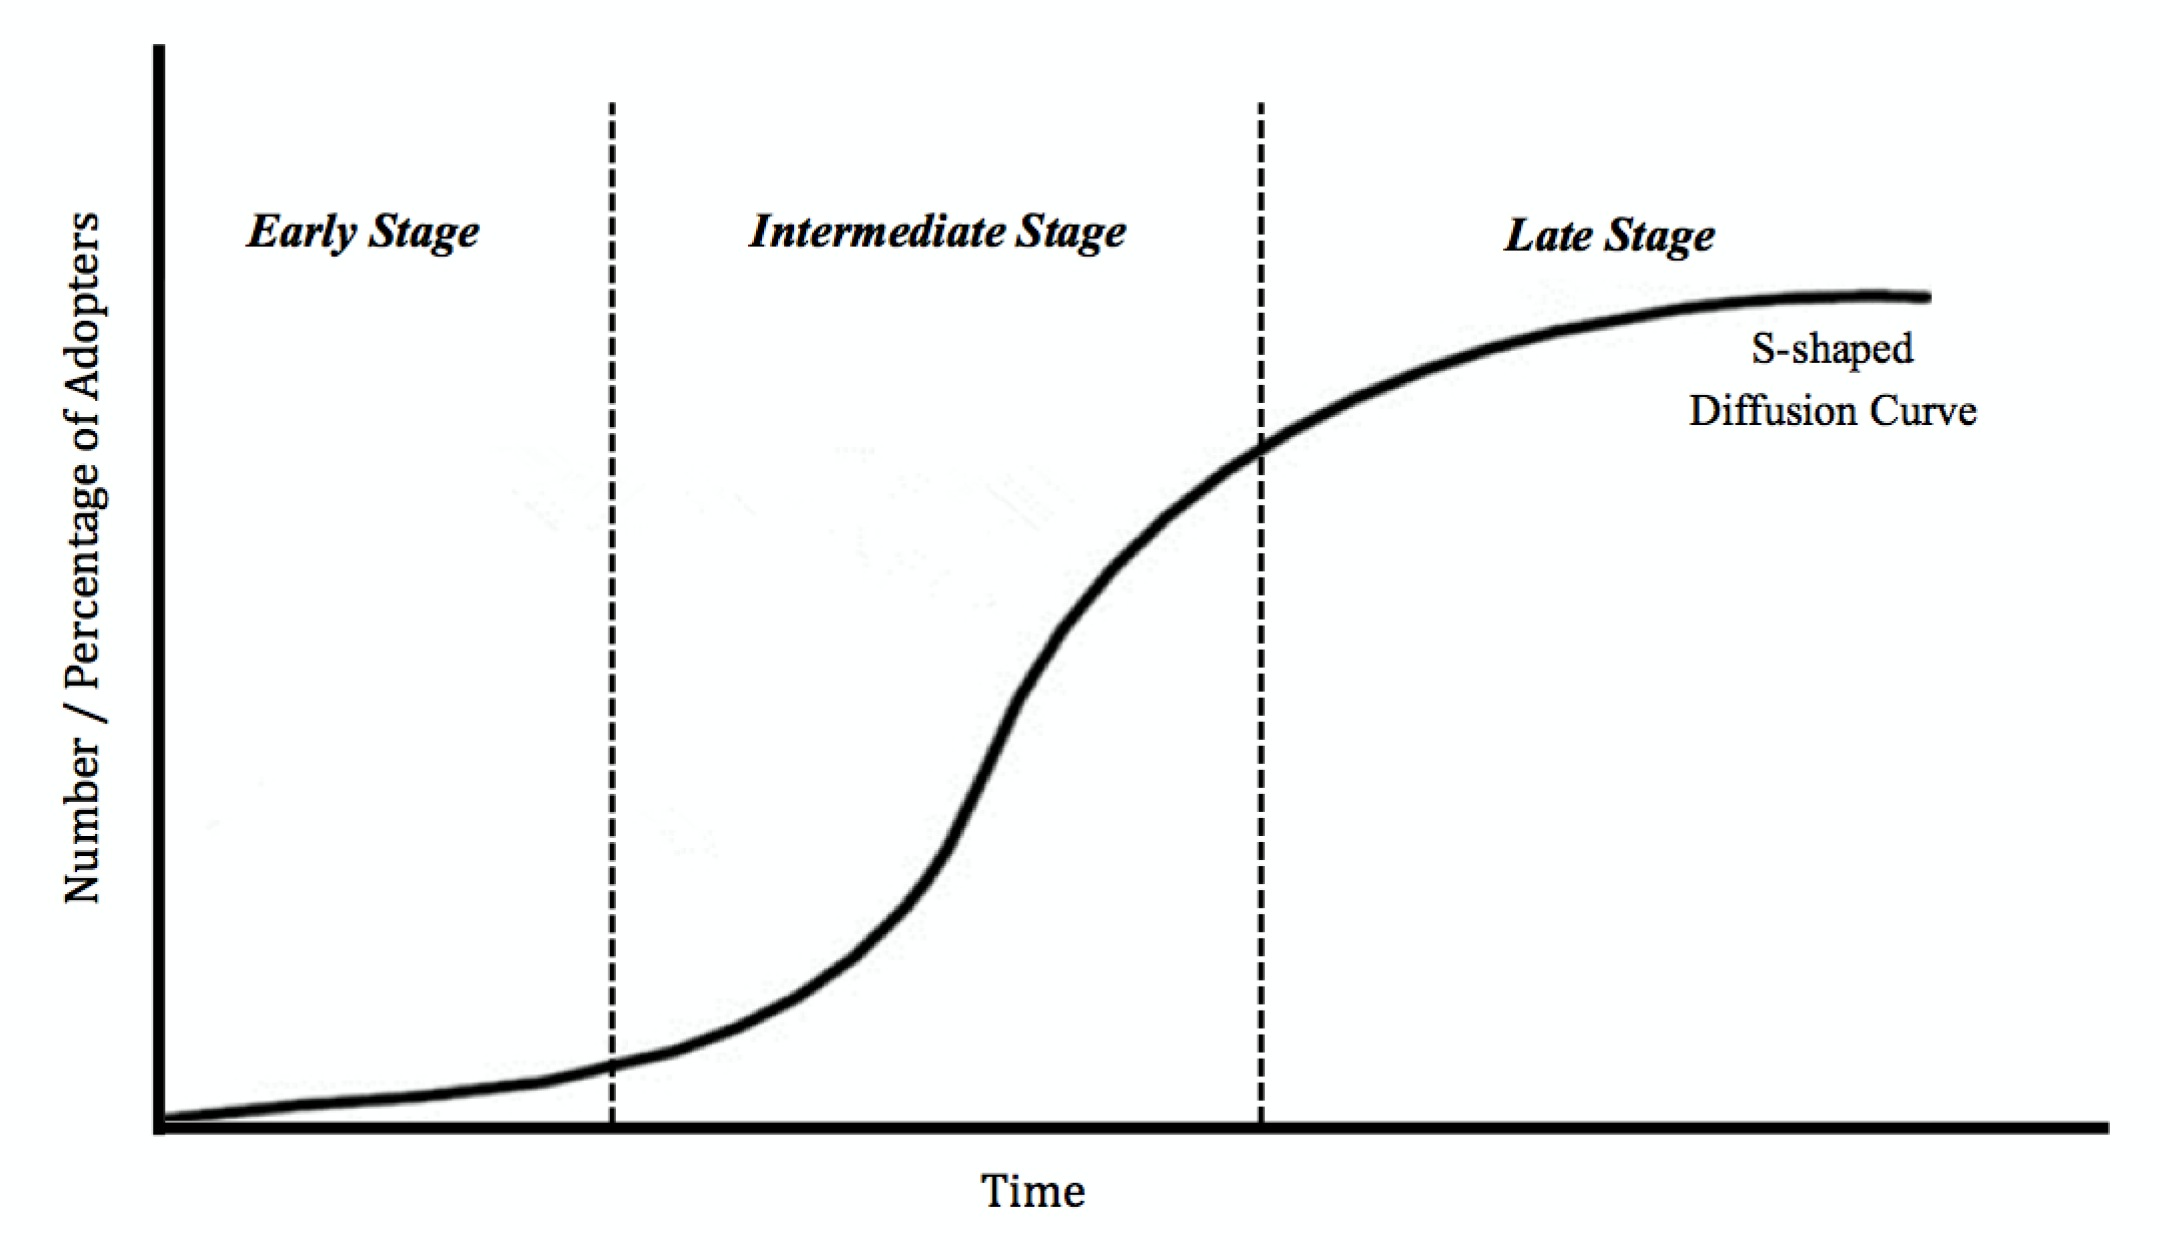
\includegraphics[scale=0.15]{peer_effects_and_diffusion_curve.jpg}
\caption{Peer Effects at Different Stages of the Diffusion Process}
\label{Fig: peer effects diffusion curve}
\end{figure}
\end{center}

Peer effects were previously either studied as a composite of different mechanisms or in a specific form (such as social leaning or network externalities). Typically only one mechanism was considered. However, a diffusion process is very often shaped by multiple mechanisms simultaneously, and each mechanism could play a different role at a different phase of the evolution of the process. Different mechanisms may potentially have different policy implications \cite{Carrell2013, Alcalde2013}. This paper is a theoretical study to examine the roles of multiple peer effects in the diffusion of innovations. We have chosen a case of the adoption of a new crop in rural China to set up our simulation model and to select key experimental parameters. In this case, all households were well informed of the new crop at the beginning of the diffusion, and thus information effect is excluded from our model. Our model and estimation are therefore focused on experience effect and externality effect.  

\section*{Background and Data}
\label{Sec: real-world case}
This paper use the case of the diffusion of a high-value crop (a crop with high economic return) in 10 villages in rural China to demonstrate multiple types of peer effects in the adoption of an innovation. The farmers in these villages traditionally farmed staple rice and cotton. The new vegetable, Artemisia selengensis (AS), was introduced into the villages in 2001. To encourage farmers to grow AS, village leaders distributed some seed-stalks to each household for free. This action informed all households about the new crop. However, as the farmers were not certain about the profitability of farming a new crop, there were only one or two households in each village (the average number of households was 37, with a standard deviation of 14) who adopted in the first year. These earlier adopters were mainly motivated by the awareness information they obtained. Their adoption behaviour was thus the result of the information effect.

When other farmers realised that farming the AS was much more profitable, they also started to farm in subsequent years. However, they encountered difficulty in obtaining seed-stalks, which can only remain fresh for a few days. It turned out that the only reliable source at the time was the earlier adopters in their villages. The seed-stalks were so scarce at the time that a household could obtain them exclusively from its close relatives. Those who managed to obtain the seed-stalks in a given year then shared them with other households next year, and so forth. Meanwhile, new adopters were often benefited by obtaining techniques and tacit knowledge from their relatives and house neighbours who have adopted earlier. Overall, the sharing of such experiential resources provided the main motivation for farmers' adoption in this stage. By 2005, more than 70\% of the households had adopted AS.

When the majority of the households by then had adopted, the non-adopters were put under some pressure to join in, mainly through the use of irrigation. There was nearly a half-year period during which both AS and cotton were active on the land. However, farming AS required much more water than farming cotton. A plot for farming cotton could thus be over flooded as its adjacent plots were planted with AS. Therefore, households farming cotton in this situation would be `coerced' into adopting AS. Such adoption was thus attributed to positive externality effect. 

\figurename \ref{Fig: diffusion curve AS} presents adoption rates of the new crop throughout the entire diffusion period. It shows an S-shaped diffusion curve as many other studies do. This case provides an excellent demonstration for the study of different types of peer effects in a complete diffusion process.

\begin{center}
\begin{figure}[ht!]
\centering
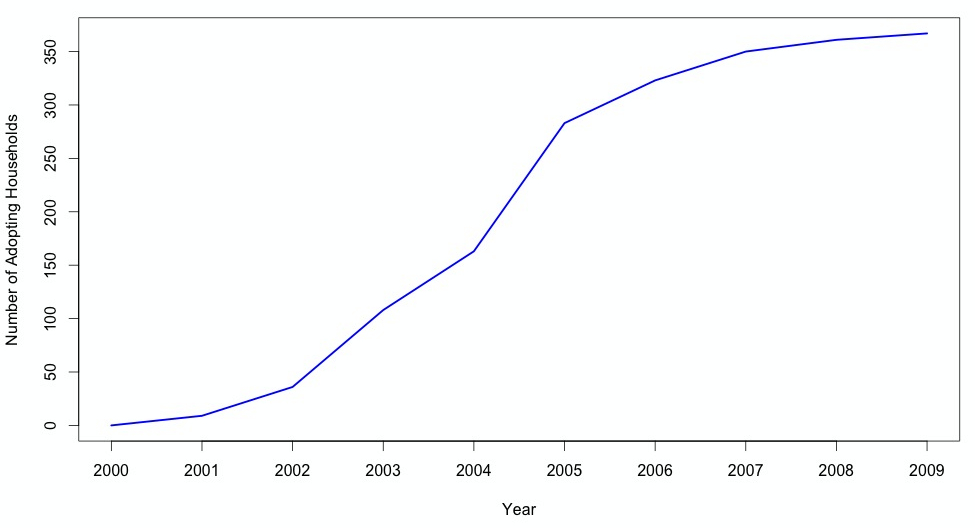
\includegraphics[scale=0.35]{Diffusion_curve_AS.jpg}
\caption{\textbf{Diffusion of the New Crop in the Chinese Villages}}
\label{Fig: diffusion curve AS}
\end{figure}
\end{center}

The data collected from this case are used to calibrate the parameters in the model. They include the number of households (i.e. nodes in the social network), characteristics of household (e.g. risk preference) ratio of initial adopters (elaborated in the section of Model Parameterisation).  

\section*{Methods and Model}
In this section, we first justify our choice of agent-based modelling for conducting this study. We then described how agents' behavioural environment (i.e., the social networks) and agents' decision-making are represented in our model. Finally, we present how parameters in the model are set up.

\subsection*{Agent-based Modelling Approach}
The underlying mechanisms following which peer effects occur in a diffusion process are generally nuanced and subtle. Empirical analysis is largely restricted because of the difficulty of data collection. Moreover, traditional approaches such as regression analysis are not capable to explicitly represent dynamic behavioural mechanisms of such. Additionally, negative peer effects in diffusions seldom enter researchers' notice. This is because failed or incomplete diffusions, which negative effects often end up with, do not draw much attention. In this study, we conducted a theoretical study following the agent-based modelling approach. This approach is able to incorporate micro-level adoption mechanisms, individuals' heterogeneity, and social relationships among individuals \cite{Kiesling2012}. Particularly for this study, it allows for the incorporation of the negative externality effect. This approach has been used to examine, for instance, the negative effects of word of mouth \cite{Goldenberg2001,Deffuant2005}.

We developed an agent-based model with peer interactions being structured in a \emph{multiplex network}; that is, a network consisting of multiple layers, on each of which a type of relationship is mapped \cite{Arenas2014}. This approach allows us to identify different peer effects in the system \cite{Bramoulle2009,Goldsmith-Pinkham2013}. To keep the model simple, we only include two effects: experience and externality. The development of our model is based on two assumptions.

Assumption 1: Peer effects exist and impose impacts on the diffusion process in the social system in study.

This assumption is made based on the theoretical analysis above as well as the observations from the real world. It permits us to circumvent the quagmire of \emph{whether} peers affect each other and be focusing on the discussion on \emph{how} this influence occurs \cite{Guryan2008}. This assumption is the prerequisite of to the simulation of the impact of peer effects, though it is often not explicitly stated in literature.
 
Assumption 2: Different types of specific peer effect (mainly) occur through different types of social relationship.

In our study, specific peer effects are distinguished according to the kind of social interactions through which they take place. It is observed that a particular type of social interaction tends to mainly take place through a particular type of social relationship (or a particular set of different types). Therefore, it is plausible that researchers are able to specify through which type(s) of relationship different specific peer effect occur in a system. This assumption enables us to model different specific peer effects on different network layers and examine how the characteristics of a network layer shape the peer effect on that layer.

\subsection*{Setup of Network Structure}
\label{simulate multiplex network}
We took the real-world case described in the section of Background and Data as a reference to design the simulation. We modelled the diffusion of the new crop using an agent-based model. In the model, the social system (environment) is village, represented as a social network. The agents were the households in the village, represented as nodes on the social network. In the villages, the interactions among households that substantially shape the diffusion mainly occurred through kinship ties, house neighbourhood ties and land plot neighbourhood ties \footnote{This is what found in the empirical study. Refer to \cite{Xiong2017} for a detailed discussion.}. 

In the model, a small portion of households are set to have adopted the innovation in the initial time. They can be considered as those adopted due to the awareness of the innovation. In other words, our model ignores information effect and focuses on experience effect and externality effect. According to the previous discussion, we reasonably assumed that experience effect occurs through kinship ties and house neighbourhood ties, whereas externality effect occurs through land plot neighbourhood ties. Since the kinship ties and house neighbourhood ties are highly overlapped in these villages (as the land for building houses were to large extent allocated based on extended family, house neighbours are often family members), we term the network consists of the two types of ties as kinship network for the sake of simplicity. The network consists of land plot neighbourhood ties is thus terms as neighbourhood network. The social network on which the peer effects occur are structured thus has two layers: the kinship network layer and the neighbourhood network layer, as demonstrated in \figurename \ref{Fig: two-layer network}. 

\begin{center}
\begin{figure}[ht!]
\centering
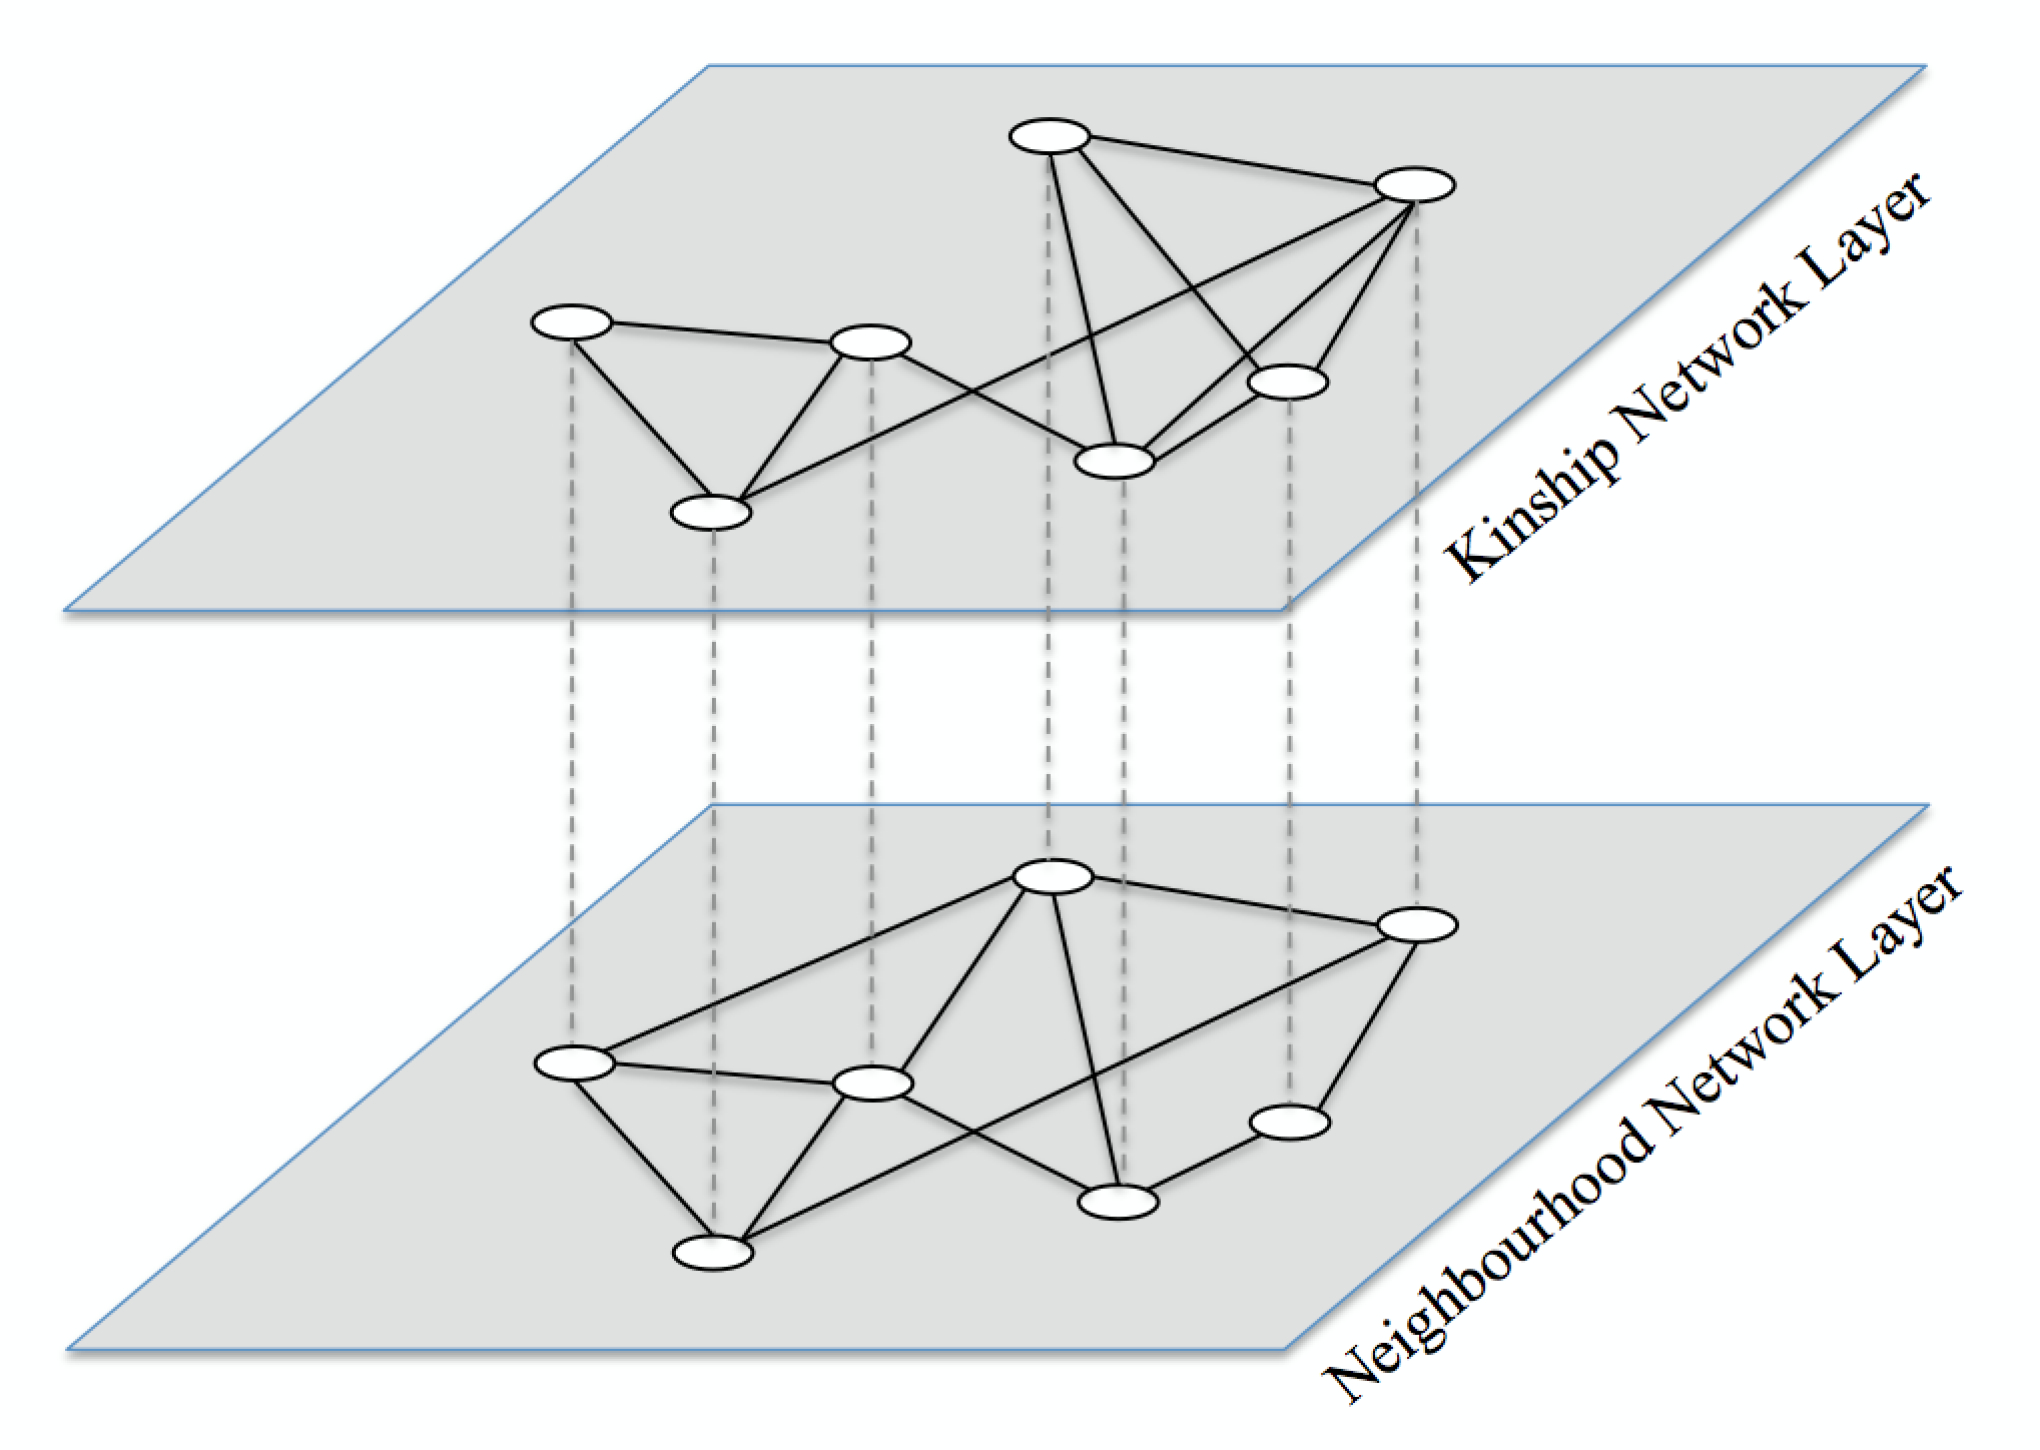
\includegraphics[scale=0.25]{two-layer_network.jpg}
\caption{Two-layer Multiplex Network}
\label{Fig: two-layer network}
\end{figure}
\end{center}

We then simulated the kinship network as a Watts-Strogatz (WS) small-world network \cite{Watts1998} and simulated the neighbourhood network as an Erd\"{o}s-R\'{e}nyi (ER) random network \cite{ErdHos1959}. These settings are reasonable. First, the kinship networks in these villages are very similar to small-world networks according the empirical study \cite{Xiong2017} and this finding echoes the classic theory of ``acquaintance society'' on the structure of traditional Chinese structure. Second, the land plot neighbourhood networks are close to random networks according to the same empirical study. This is the case because the plots were originally distributed by lot. The parameters defining the network structures were roughly calibrated according to the network characteristics of the villages in our real-world case. 

\subsection*{Simulation of Agents' Decision-making}
Two approaches are widely utilised to describe diffusion in social groups. One is a probability-based approach (e.g., \cite{Banerjee2013,Peres2014}), where individuals' probability of adopting the innovation increases as the fraction of peers that adopt increase. The other is a threshold-based approach (e.g., \cite{Granovetter1978,Singh2013}), where individuals change their adoption state when a certain threshold of utility is reached. In the case of this study, on the kinship network, the more an individual's peers have adopted the new crop, the more likely that the individual gains information and thus follow suit. We therefore simulated experience effect on the kinship network following the probability-based approach. The probability for an individual to adopt is proportional to the fraction of his family members who have adopted. Meanwhile, the externalities of planting the new crop are mainly determined by the nature of the crop itself, such as its compatibility with the existing crop. This can be viewed as a threshold that all practitioners face. Once the fraction of one's neighbours who adopt reaches the threshold, an individual will adopt for sure. Thus, the externality effect occurring on the neighbourhood network is modelled using a threshold.

Suppose there are $N$ nodes in the network, i.e., on each of the two layers. On the kinship network, node (household) $i$ chooses to adopt the innovation with a probability $p_{i}$. The probability is determined by the fraction of his adopting peers $f_i^{kin}$ as well as his risk preference (a representative of the individual's personal characteristics) $x_{i} \in (0,1)$. Therefore, $p_{i} = \theta f_i^{kin} x_i$, where $\theta \in (0,1)$ is a coefficient indicating the degree of information effect (namely \emph{information coefficient}). On the neighbourhood network, household $i$ changes his adoption state when the fractions of his adopting neighbours $f_i^{geo}$ reaches a unified adoption threshold (namely \emph{externality threshold}, denoted by $\delta$), which is determined by the characteristics of the new crop. When the threshold is reached, in the scenario of the positive externality effect, the \emph{non-adopters} switch to adopting state; in the scenario of negative externality effect, the \emph{adopters} change back to non-adopting. 

A household has two adoption status: \emph{Adopting} or \emph{non-adopting}. We track households' adoption states and the ratio of adopting households (namely the \emph{adoption rate}) at the village level. The basic algorithm of the simulation is as follows:

\begin{enumerate}
\item [(i)] Initial time $t=0$

A fraction $\lambda$ of seed adopters is selected from the population of the households at random. Meanwhile, their adoption states are set to be adopting.

\item [(ii)] Iteration at time $t$, 

Households update their state through kinship ties and neighbourhood ties simultaneously. 
\begin{itemize}
\item [(a)] Updating on the kinship network

The non-adopters adopt with probability $p_{it} = \theta f_{it}^{kin} x_{i}$.

\item [(b)]Updating on the neighbourhood network

In the scenario of positive externality effect, non-adopting household $i$ transmits to adopting state once the fraction of his adopting neighbours reaches the externality threshold, i.e., $f_{it}^{geo} > \delta$. 

In the case of negative externality effect, adopting household $i$ transmits to non-adopting state once the fraction of his adopting neighbours reaches the externality threshold, i.e., $f_{it}^{geo} > \delta$. 
\end{itemize}
\end{enumerate}

The two updating mechanisms occur simultaneously in reality, so we set the order to be random when updating on the two layers in the model. The process repeats until any of the following termination rules is satisfied: (i) the adoption rate is lower than $5\%$ (which is the lowest ratio of seed adopters), (ii) the adoption rate is higher than $95\%$ (i.e., complete diffusion), and (iii) it iterates for 20 times -- this is sufficient for the system to converge in most cases (both in the simulation and in the real world).

\subsection*{Model Parameterisation}
\label{parameterisation}
The parameters in the simulation model are set using the survey data from the 10 reference villages. Parameter values are set to the mean estimates from the data. The parameters were set up as follows:
\begin{itemize}
\item Number of nodes (the population) $N\in [20 : 20 : 80]$

\item Fraction of rewiring nodes in the generation of WS small-world networks $WS_f\in \{0.05, 0.s, 0.15\}$

\item Rewiring probability in the generation of ER random networks $ER_{prob} \in \{0.10, 0.15, 0.20\}$

\item Experience coefficient $\theta \in [0.05 : 0.05 : 0.25]$

\item Externality threshold $\delta \in [0.6 : 0.05 : 0.80]$ 

\item Ratio of seed adopters $s \in [0.05 : 0.05 : 0.20]$

\item Risk preference of household $i$, $x_i$. The value is generated as a positive random number with normal distribution (mean $1$ and standard deviation $0.3$; truncated to 0 and 2 for values less than 0 and greater than 2 respectively).
\end{itemize}

We run each parameter combination 100 times. There are 3,600 (full factorial) combinations in total, and the model runs each of these combinations 100 times. Finally, 360,000 sets of simulation results were generated.

\section*{Results}
\subsection*{Convergence Adoption Rates and Diffusion Curves}
\subsubsection*{Scenario of Positive Externality Effect}
\paragraph{Convergence Adoption Rates} 
The densities of convergence adoption rates and convergence rounds are presented in \figurename \ref{Fig: hist conv adp and round pos}. The left panel shows that approximately 85\% of the runs converge to \emph{full adoption} (that is, as we defined, more than 90\% of the population have adopted) within 20 iterations. It means that most individuals adopt eventually. The right panel indicates how many rounds it takes for the runs to converge. More than 40\% of the runs converge in five rounds. The density decreases with the number of rounds\footnote{The density at the 20th round is as high as over 15\% because it also contains the cases that take more than 20 rounds to converge and those do not converges to full adoption.}. In this scenario, both the two diffusion mechanisms are positive feedback mechanisms, so it is very likely that the system will converge to complete diffusion.

\begin{center}
\begin{figure}[ht!]
\centering
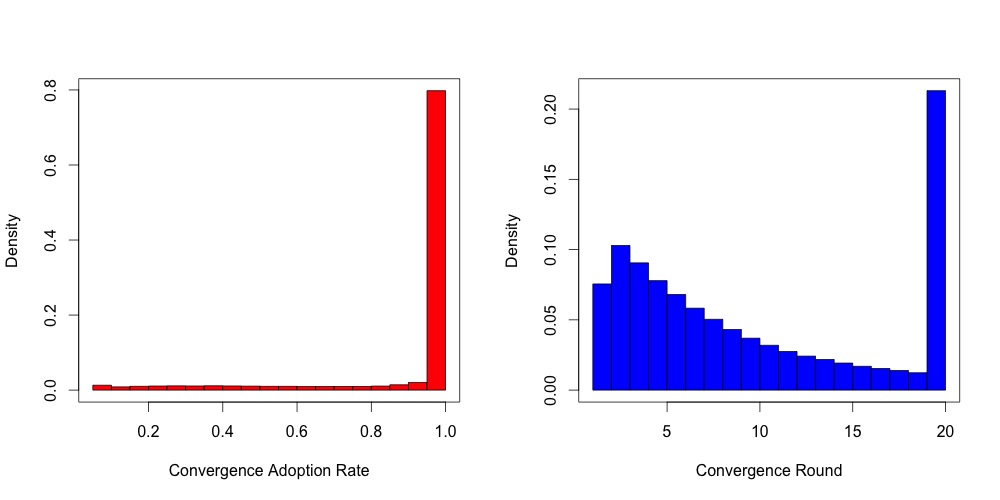
\includegraphics[scale=0.35]{Hist_conv_adp_and_round_pos.jpg}
\caption{\textbf{Histogram of Convergence Adoption Rates and Convergence Rounds (Positive Externality Effect)}}
\label{Fig: hist conv adp and round pos}
\end{figure}
\end{center}

\paragraph{S-shaped Diffusion Curves}
The S-shaped adoption curve is a typical pattern of the diffusion. It holds because most innovations bear the following feature: The adoption rate grows slowly at the beginning of the diffusion process. When the diffusion reaches the \emph{critical mass}, it will have a sharp increase. After that it will slowly approach complete diffusion. The variance lies in the slope of the curve. The innovations diffusing rapidly generate steep curves, whereas those diffusing slowly generate flat curves. Our simulations successfully generate S-shaped diffusion curves. \figurename \ref{Fig: s-shaped curves round=6} displays the curves for the diffusions converge at the 6th round, and the ratio of seed adopters is 0.05 and 0.1, respectively\footnote{To have a better visualisation, we average the adoption rates over repetitive runs. The speed at which the adoption rate grows varies significantly over different settings, so a fat midsection of the integrated graph is observed when plotting all the curves in one frame of axes.}.

\begin{center}
\begin{figure}[ht!]
\centering
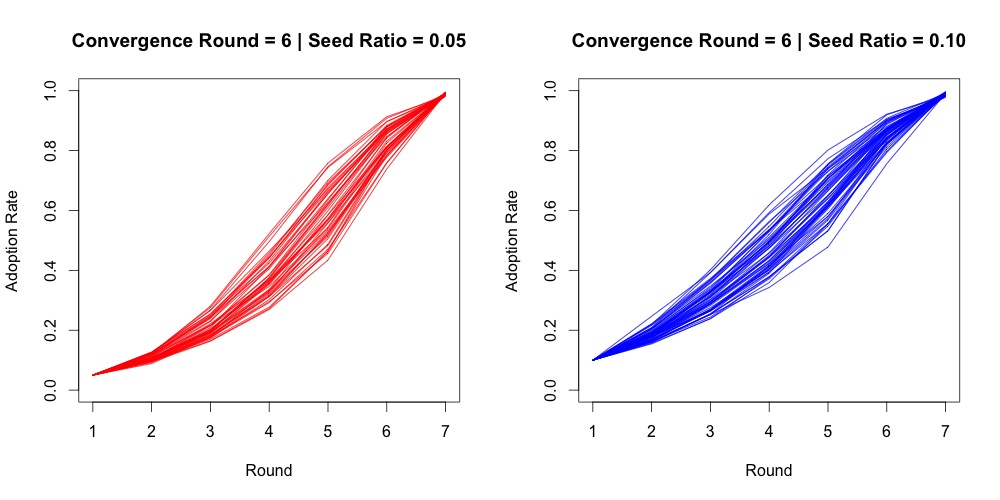
\includegraphics[scale=0.35]{S-shape_curves_round_6_pos.jpg}
\caption{S-shaped Diffusion Curves (Convergence Round = 6)}
\label{Fig: s-shaped curves round=6}
\end{figure}
\end{center}

\subsubsection*{Scenario of Negative Externality Effect}
\paragraph{Convergence Adoption Rates}
The diffusion converges to diverse adoption rates in this scenario. As shown in \figurename \ref{Fig: hist conv adp and round neg}, nearly $70\%$ of the simulations converge to an adoption rates between $40\%$ and $80\%$. Specifically, more than $25\%$ converge to a value in the interval of $50\%-60\%$ and more than $25\%$ converge to a value between $60\%$ and $70\%$. Only about $5\%$ end up with full adoption. More than $90\%$ of the simulations converged within 20 rounds.

\begin{center}
\begin{figure}[ht!]
\centering
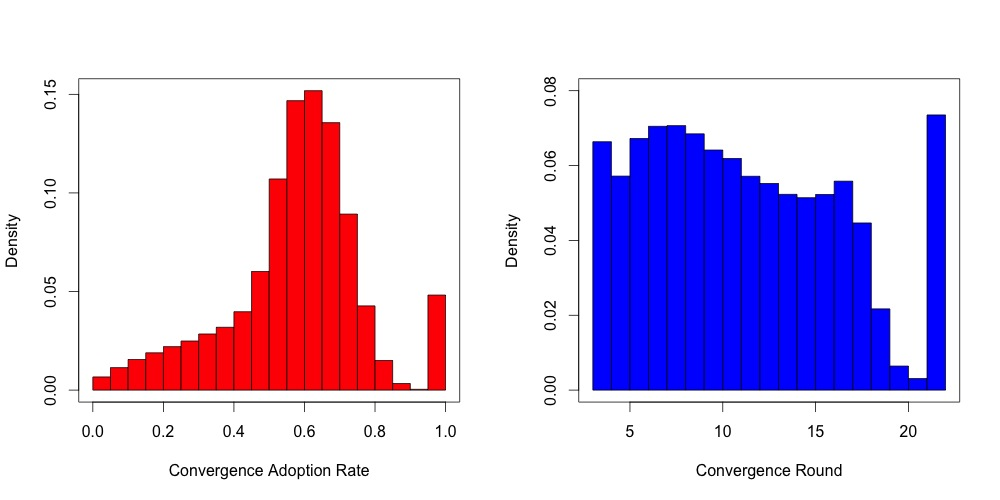
\includegraphics[scale=0.35]{Hist_conv_adp_and_round_neg.jpg}
\caption{Histogram of Convergence Adoption Rates and Convergence Rounds (Negative Externality Effect)}
\label{Fig: hist conv adp and round neg}
\end{figure}
\end{center}

When a negative effect is introduced, the diffusion curve dramatically changes its shape. Converging to full adoption is not a certain outcome any more. At which adoption rate the diffusion will converge depends on the competition between the positive effect and the negative effect. This result provides an interpretation of the incomplete diffusion phenomena in the real world. For instance, in the case of mircofinance \cite{Banerjee2013}, the average take-up rate is $18.5\%$ over all rural communities that were studied. Most innovations end up with not been taken up by the all potential adopters in the social group. New fashionable clothes can be a typical example. When they go from high fashion to street fashion, they are not considered fashionable any more, and thus become less attractive. This negative effect leads the diffusion to converge before reaching full adoption.

\paragraph{Fluctuating Diffusion Curves}

\figurename \ref{Fig: fluctuating curves round=6} displays the diffusion curves for the simulations that converge, again, at the 6th round with the ratios of seed adopters 0.05 and 0.1, respectively. To exhibit the trends of the curves, the adoption rates after the convergence are also plotted. The graph shows that the diffusion curves fluctuate around a value in the middle of 0 and 1 (approximately $0.6$ in our case). The specific convergence value depends on the relative strength of the two opposite effects in the diffusion process.

\begin{center}
\begin{figure}[ht]
\centering
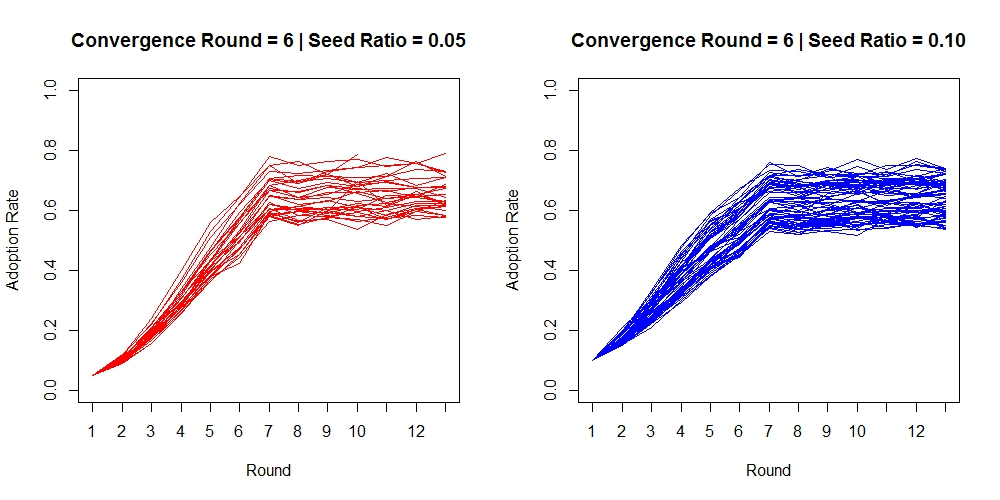
\includegraphics[scale=0.35]{Fluctuating_curves_round_6_neg.jpg}
\caption{Fluctuating Diffusion Curves (Convergence Round = 6)}
\label{Fig: fluctuating curves round=6}
\end{figure}
\end{center}

Overall, when all specific diffusion mechanisms in the system are in favour of diffusion, the system will almost always converge to complete diffusion, and an S-shaped diffusion curve will be generated. When there is a negative mechanism, it reshapes the diffusion to fluctuate around a middle-level rate, hence generating fluctuating diffusion curves.

\subsection*{Experience Effect and Externality Effect}
We explore how experience effect and externality effect influence the effectiveness of diffusion, which is measured by the reach of the diffusion and its speed. The two measures are both related to \emph{adoption rate}, the fraction of households that have adopted at a round to the whole population. Specifically, \emph{convergence adoption rate}, reflecting the reach of the diffusion, is defined as the adoption rate at which the diffusion converges. \emph{Diffusion speed} is defined as the increase of the adoption rate per round, or namely, the expression of the adoption rate achieved by the number of rounds to achieve it\footnote{To measure the number of rounds over all runs with a unified standard, we split the values of adoption rate into 10 diffusion bins. The values higher then 10\% and less than 20\% are in the 10\% bin, those higher than 20\% and less than 30\% are in the 20\% bin, and so on, up to the 90\% bin. For instance, it takes 4 rounds for the diffusion to first achieve the diffusion level of, say, 58\%. The actual adoption rate at the 4th round is 58\%. Suppose the seed ratio is 10\%, then the growth rate for the system to achieve 50\% diffusion in this setting is $(58\%-10\%)/4=12\%$. There are cases that the diffusion speed is the same for several diffusion bins. For instance, suppose the adoption rate jumps from 34\% to 66\% at the fourth round, and the seed ratio is 10\%, the diffusion speed for the 30\% bin is thus $(34\%-10\%)/3=8\%$, and that for the 40\%, 50\% and 60\% bins are all $(66\%-10\%)/4=14\%$.}. However, the two metrics cannot be both used in positive and negative externality effect at the same time. When the externality effect is positive, the diffusion almost always converges to $100\%$, so the convergence adoption rate is not a feasible metric. Likewise, the diffusion speed does not apply when the externality effect is negative because the adoption rate oscillates over the diffusion process, but we can use \emph{convergence speed} (how fast the diffusion process converges) as a substitute. It is the quotient of convergence adoption rate by the number of rounds it takes to achieve the rate. Therefore, the diffusion speed is used in the scenario of positive externality effect, whereas the convergence adoption rate and convergence speed are employed in the scenario of negative externality effect.

In the model, the experience effect and the externality effect are reflected by the experience coefficient and the externality threshold, respectively. Higher experience coefficient indicates higher experience effect, whereas higher externality threshold indicates lower externality effect. To estimate their impact on the effectiveness of diffusion, we run a multivariate regression using the following equation:
\begin{equation}
\label{Eq: peer effects}
y=\alpha_0 + \alpha_1 \theta + \alpha_2 \delta + \alpha_3s+ W' \alpha_4 + \epsilon
\end{equation}
where $y$ is the diffusion speed (in the scenario of positive externality effect) or the convergence adoption rate (in the scenario of negative externality effect),  $\theta$ is the experience coefficient, $\delta$ is the externality threshold, $s$ is the ratio of initial seed adopters and $W'$ is the network characteristic controls, including number of nodes $N$, parameters used in generating ER network (i.e., rewiring probability $ER_{prob}$) and WS network (i.e., fraction of rewiring nodes $WS_f$).

We note that the traditional null hypothesis test is not well suited for simulation studies because with a sufficient number of simulated trajectories one can make the p-value arbitrarily small \cite{Heard2014}. Thus, we conduct a traditional minimum-effect test. We test that the difference is bigger than an a priori defined minimal meaningful effect (MME). Parameter values significantly smaller than the MME signify no effect. Parameter values significantly large than MME signify significant difference, and when the statistical significance is not achieved it signifies that no conclusion could be made given the data. Under such paradigm the increase in the number of simulations will increase the precision and reduce the p-values but will not produce artificially significant small effect sizes \cite{Wellek2010}. Such approach is also the basis for a classic power analysis, which requires to explicitly define a minimally meaningful effect size. In our study we have selected the MME to be 0.1 standard deviation. Our judgement on the significance of estimated values in the regression results in this study are based on the minimum-effect test (whether they are significantly larger than the minimal effect defined as 0.1 of the standard deviation).

\subsubsection*{Scenario of Positive Externality Effect}
\label{Sec: experience effect and externality effect pos}
We regress the diffusion speed when the adoption rate reaches 30\%, 40\%, up to 90\%. \tablename \ref{Tab: reg adoption speed pos} presents the results\footnote{All effect sizes reported in the table were significantly larger than the minimally meaningful effect of 0.1 standard deviations. This is the same for all the following tables that report regression results.}. First, all the estimated values were significantly larger than the minimal effect defined as 0.1 of the standard deviation. Specifically, both the experience coefficient and the externality threshold in the simulation are highly significantly associated with the diffusion speeds, and the signs are in accordance with expectations. This indicates that they both impose a significant influence on the diffusion. More importantly, we found the influence of the experience effect wanes as the adoption rate increases (i.e., the diffusion process), while the influence of the externality effect continuously grows. At the earlier stage, the adopters are few, so only a small number of households can reach the externality thresholds. Consequently, the externality effect has a limited impact on the diffusion. Meanwhile, the experience effect, which is continuous and steady, has a major contribution. At the later stage, there are more adopters, thus more households can reach the externality threshold. Externality effect, therefore, become relatively higher. However, this could undermine the influence of experience effect, because the two effects can substitute each other -- a household can make the adoption decision because of either experience effect or externality effect. Such a substitution effect becomes larger as the adoption rate increases.

\begin{table}
\begin{center}
\caption{Regression for Adoption Speeds at Different Diffusion Levels (Positive Externality Effect)}
\label{Tab: reg adoption speed pos}
\resizebox{\linewidth}{!}{
\begin{tabular}{l D{.}{.}{5}@{} D{.}{.}{5}@{} D{.}{.}{5}@{} D{.}{.}{5}@{} D{.}{.}{5}@{} D{.}{.}{5}@{} D{.}{.}{5}@{} }
\toprule
\hline
& \multicolumn{1}{c}{Model 1} & \multicolumn{1}{c}{Model 2} & \multicolumn{1}{c}{Model 3} & \multicolumn{1}{c}{Model 4} & \multicolumn{1}{c}{Model 5} & \multicolumn{1}{c}{Model 6} & \multicolumn{1}{c}{Model 7} \\
& \multicolumn{1}{c}{(30\%)$^{*}$} & \multicolumn{1}{c}{(40\%)} & \multicolumn{1}{c}{(50\%)} & \multicolumn{1}{c}{(60\%)} & \multicolumn{1}{c}{(70\%)} & \multicolumn{1}{c}{(80\%)} & \multicolumn{1}{c}{(90\%)} \\
\midrule
(Intercept)                       & -0.53 & -0.50 & -0.47 & -0.45 & -0.43 & -0.32 & -0.32 \\
Number of Households                   & 0.01  & 0.01  & 0.01  & 0.01  & 0.01  & 0.01  & 0.01  \\
Ratio of Seed Adopters               & 0.90  & 0.84  & 0.81  & 0.80  & 0.78  & 0.57  & 0.57  \\
Experience Coefficient            & 2.04  & 2.02  & 2.01  & 1.99  & 1.94  & 1.54  & 1.54  \\
Externality Threshold             & -0.18 & -0.21 & -0.23 & -0.25 & -0.26 & -0.28 & -0.28 \\
\% of Neighbours to Connect in WS & 3.23  & 3.24  & 3.23  & 3.21  & 3.16  & 2.53  & 2.53  \\
Rewiring Probability in ER        & -0.15 & -0.14 & -0.12 & -0.10 & -0.08 & 0.09  & 0.09  \\
\midrule
R$^2$                             & 0.75      & 0.78        & 0.80        & 0.80        & 0.80        & 0.72        & 0.72        \\
\hline
\bottomrule
\multicolumn{8}{l}{\small{$^*$ The adoption rate level for diffusion speed in the present regression. This is the same for \tablename \ref{Tab: reg peer effects average degree pos}, \ref{Tab: reg peer effects clustering coefficient pos} and \ref{Tab: reg peer effects average path length pos}.}}
%\multicolumn{8}{l}{\small{\dag All effect sizes were significantly larger than the minimally meaningful effect of 0.1 standard deviations.}}
\end{tabular}
}
\end{center}
\end{table}

\subsubsection*{Scenario of Negative Externality Effect}
\label{Sec: experience effect and externality effect neg}
We run the regression also using the equation (\ref{Eq: peer effects}). The same explanatory variables as in the scenario of positive externality effect (the experience coefficient, the externality threshold, the ratio of initial seed adopters, and the network characteristics) are employed. They are regressed against two response variables, the convergence adoption rate (Model 1 in \tablename \ref{Tab: reg adoption rate neg}) and the convergence speed (Model 2 in \tablename \ref{Tab: reg adoption rate neg}). The results show that both the experience effect and the externality effect are significantly correlated to these response variables with expected signs, suggesting that they both have significant impacts on diffusion\footnote{The quality of fit for the models using convergence adoption rate as the response variable (Model 1 in \tablename \ref{Tab: reg adoption rate neg}, \ref{Tab: reg peer effects average degree neg}, \ref{Tab: reg peer effects clustering coefficient neg} and \ref{Tab: reg peer effects average path length neg}) is low. Other factors or non-linear structures could provide a better model fit. However in here we have focused on specific models, and the exploration of the best fitted models is beyond the scope of the study.}. 

\begin{table}
\begin{center}
\caption{Regression on Convergence Adoption Rate and Convergence Speed (Negative Externality Effect)}
\resizebox{0.8\linewidth}{!}{
\label{Tab: reg adoption rate neg}
\begin{tabular}{l D{.}{.}{15}@{} D{.}{.}{15}@{} }
\toprule
\hline
& \multicolumn{1}{c}{Model 1} & \multicolumn{1}{c}{Model 2} \\
& \multicolumn{1}{c}{(Conv. Adp. Rate)} & \multicolumn{1}{c}{(Conv. Speed)} \\
\midrule
(Intercept)                       & 0.90  & -0.31 \\
Number of Households                   & 0.00  & 0.01  \\
Ratio of Seed Adopters               & 0.17  & 0.57  \\
Experience Coefficient            & 0.19  & 1.53  \\
Externality Threshold             & -0.05 & -0.28 \\
\% of Neighbours to Connect in WS & 0.39  & 2.53  \\
Rewiring Probability in ER        & -0.02 & 0.06  \\
\midrule
R$^2$                             & 0.11        & 0.72        \\
\hline
\bottomrule
\end{tabular}
}
\end{center}
\end{table}

\subsection*{Network Characteristics and Peer Effects}
\label{Sec: network characteristics and peer effects}
The diffusion of innovation is usually influenced by the structure of the network in which it takes place \cite{Peres2014}. We measure the structure of the networks used in our simulation using three metrics: average degree, clustering coefficient and average path length. They are chosen because they reflect different aspects of the characteristics of a network: Average degree indicates how connected the network is (i.e., the connectivity); clustering coefficient measures how clustered the nodes are and thus how well the information can transmit (i.e., the transitivity); and average path length represents how many intermediaries it needs for one node to reach another (i.e., the network distance).

To estimate the impact of these network topological metrics on the corresponding network layer, we introduce a interaction term into the regressions. The interaction term is generated by multiplying the experience coefficient or the externality threshold by each of the topological metrics on the corresponding network layer. The interaction effect can be interpreted from the regression coefficients of the interaction terms. As different topological metrics and the network generation parameters are highly correlated with each other (as presented in \tablename \ref{Tab: correlation network characteristics pos} for the scenario of positive externality effect, and those for the scenario of negative externality effect are similar), we run the regression for each topological metric separately (and drop the network generation parameters served as controls). 


\begin{table}
\begin{center}
\caption{Correlations between Network Characteristics (Positive Externality Effect)}
\label{Tab: correlation network characteristics pos}
\resizebox{0.9\linewidth}{!}{
\begin{tabular}{l D{.}{.}{5}@{} D{.}{.}{5}@{} D{.}{.}{5}@{} D{.}{.}{5}@{} D{.}{.}{5}@{} D{.}{.}{5}@{} D{.}{.}{5}@{} D{.}{.}{5}@{} }
\toprule
\hline
&(Var 1) & (Var 2) & (Var 3) &  (Var 4) & (Var 5) & (Var 6) & (Var 7) & (Var 8)\\ 
\midrule
$WS_f$ & 1 &  &  &  &  &  &  & \\ 
Avg. Dg. of Kin. & 0.65 & 1 &  &  &  &  &  &  \\ 
Clu. Coef. of Kin. & 0.83 & 0.69 & 1 &  &  &  &  &  \\ 
APL of Kin. & -0.73 & -0.64 & -0.86 & 1 &  &  &  & \\ 
$ER_{prob}$ &  &  &  &  & 1 &  &  &  \\ 
Avg. Dg. of Nei. &  &  &   &  & 0.49 & 1 &  &  \\ 
Clu. Coef. of Nei. &  &  &  &  & 0.71 & 0.43 & 1 &  \\
APL of Nei. &  &  &  & & -0.65 & -0.76 & -0.58 & 1 \\
\hline
\bottomrule
\end{tabular}
}
\end{center}
\end{table}

The resultant regression equation is the following:

\begin{equation}
\label{Eq: peer effects and network characteristics}
y=\beta_0 + \beta_1 \theta + \beta_2 \delta + \beta_3 Net\_char + \beta_4 Inter\_term + \beta_5s+ \epsilon
\end{equation}
where $Net\_char$ denotes the vector of topological metrics on the kinship network and the neighbourhood network, respectively; and $Inter\_term$ denotes the vector of interaction terms. The interaction term is the product of a topological metric and the corresponding peer effect indicator occurring on the network. For instance, the interaction term of average degree and peer effect on kinship network is $(average\; degree\; of\; kinship\; network)\times \theta$. One topological metric is run for each regression. As there are two scenarios, the regression runs in a total of 6 times ($3 \times 2$).

\subsubsection*{Scenario of Positive Externality Effect}
As discussed previously, we use the diffusion speed as the response variable in the regressions. Results for average degree, clustering coefficient and average path length are displayed in \tablename \ref{Tab: reg peer effects average degree pos}, \ref{Tab: reg peer effects clustering coefficient pos} and \ref{Tab: reg peer effects average path length pos}, respectively. 

\begin{table}
\begin{center}
\caption{Peer Effects and Average Degree (Positive Externality Effect)}
\label{Tab: reg peer effects average degree pos}
\resizebox{\linewidth}{!}{
\begin{tabular}{l D{.}{.}{5}@{} D{.}{.}{5}@{} D{.}{.}{5}@{} D{.}{.}{5}@{} D{.}{.}{5}@{} D{.}{.}{5}@{} D{.}{.}{5}@{} }
\toprule
\hline
& \multicolumn{1}{c}{Model 1} & \multicolumn{1}{c}{Model 2} & \multicolumn{1}{c}{Model 3} & \multicolumn{1}{c}{Model 4} & \multicolumn{1}{c}{Model 5} & \multicolumn{1}{c}{Model 6} & \multicolumn{1}{c}{Model 7} \\
& \multicolumn{1}{c}{(30\%)} & \multicolumn{1}{c}{(40\%)} & \multicolumn{1}{c}{(50\%)} & \multicolumn{1}{c}{(60\%)} & \multicolumn{1}{c}{(70\%)} & \multicolumn{1}{c}{(80\%)} & \multicolumn{1}{c}{(90\%)} \\
\midrule
(Intercept)                    & -0.07 & -0.05 & -0.04 & -0.03 & -0.01  & 0.02  & 0.02  \\
Number of Households           & -0.00 & 0.00        & 0.00  & 0.00  & 0.00  & 0.00  & 0.00  \\
Ratio of Seed Adopters                     & 0.90  & 0.84  & 0.81  & 0.80  & 0.78  & 0.57  & 0.57  \\
Experience Coefficient (Var 1)        & 0.87  & 0.99  & 1.07  & 1.08  & 1.02  & 0.74  & 0.74  \\
Externality Threshold (Var 2)         & -0.16 & -0.19 & -0.21 & -0.23 & -0.23 & -0.22 & -0.22 \\
Average Degree of Kin. (Var 3)      & 0.01  & 0.01  & 0.02  & 0.02  & 0.01  & 0.01  & 0.01  \\
Average Degree of Nei. (Var 4) & -0.00       & 0.00        & 0.00        & 0.00    & 0.00  & 0.01  & 0.01  \\
Var 1 $\times$ Var 3                  & 0.12  & 0.10  & 0.10  & 0.09  & 0.09  & 0.08  & 0.08  \\
Var 2 $\times$ Var 4             & -0.01 & -0.00 & -0.00 & -0.00 & -0.00 & -0.01 & -0.01 \\
\midrule
R$^2$                          & 0.80        & 0.81        & 0.82        & 0.82        & 0.82        & 0.75        & 0.75        \\
\hline
\bottomrule
\end{tabular}
}
\end{center}
\end{table}


\begin{table}
\begin{center}
\caption{Peer Effects and Clustering Coefficient (Positive Externality Effect)}
\label{Tab: reg peer effects clustering coefficient pos}
\resizebox{\linewidth}{!}{
\begin{tabular}{l D{.}{.}{5}@{} D{.}{.}{5}@{} D{.}{.}{5}@{} D{.}{.}{5}@{} D{.}{.}{5}@{} D{.}{.}{5}@{} D{.}{.}{5}@{} }
\toprule
\hline
& \multicolumn{1}{c}{Model 1} & \multicolumn{1}{c}{Model 2} & \multicolumn{1}{c}{Model 3} & \multicolumn{1}{c}{Model 4} & \multicolumn{1}{c}{Model 5} & \multicolumn{1}{c}{Model 6} & \multicolumn{1}{c}{Model 7} \\
& \multicolumn{1}{c}{(30\%)} & \multicolumn{1}{c}{(40\%)} & \multicolumn{1}{c}{(50\%)} & \multicolumn{1}{c}{(60\%)} & \multicolumn{1}{c}{(70\%)} & \multicolumn{1}{c}{(80\%)} & \multicolumn{1}{c}{(90\%)} \\
\midrule
(Intercept)                    & -0.17 & -0.17 & -0.17 & -0.16 & -0.15 & -0.08 & -0.08 \\
Number of Households           & 0.00  & 0.00  & 0.00  & 0.00  & 0.00  & 0.00  & 0.00  \\
Ratio of Seed Adopters                     & 0.91  & 0.84  & 0.81  & 0.80  & 0.78  & 0.57  & 0.57  \\
Experience Coefficient (Var 1)        & 0.21  & 0.35  & 0.43  & 0.45  & 0.41  & 0.31  & 0.31  \\
Externality Threshold (Var 2)         & -0.18 & -0.20 & -0.21 & -0.22 & -0.23 & -0.25 & -0.25 \\
Clustering Coefficient of Kin. (Var 3)     & 0.12  & 0.22  & 0.29  & 0.31  & 0.30  & 0.24  & 0.24  \\
Clustering Coefficient of Nei. (Var 4) & -0.10   & -0.03      & 0.04        & 0.07    & 0.12   & 0.22  & 0.22  \\
Var 1 $\times$ Var 3                  & 7.06  & 6.47  & 6.10  & 5.9  & 5.80  & 4.77  & 4.77  \\
Var 2 $\times$ Var 4           & -0.00       & -0.08       & -0.16  & -0.20 & -0.24 & -0.25 & -0.25 \\
\midrule
R$^2$                          & 0.70        & 0.72        & 0.74        & 0.75        & 0.75        & 0.68        & 0.68        \\
\hline
\bottomrule
\end{tabular}
}
\end{center}
\end{table}

\begin{table}
\begin{center}
\caption{Peer Effects and Average Path Length (Positive Externality Effect)}
\label{Tab: reg peer effects average path length pos}
\resizebox{\linewidth}{!}{
\begin{tabular}{l D{.}{.}{5}@{} D{.}{.}{5}@{} D{.}{.}{5}@{} D{.}{.}{5}@{} D{.}{.}{5}@{} D{.}{.}{5}@{} D{.}{.}{5}@{} }
\toprule
\hline
& \multicolumn{1}{c}{Model 1} & \multicolumn{1}{c}{Model 2} & \multicolumn{1}{c}{Model 3} & \multicolumn{1}{c}{Model 4} & \multicolumn{1}{c}{Model 5} & \multicolumn{1}{c}{Model 6} & \multicolumn{1}{c}{Model 7} \\
& \multicolumn{1}{c}{(30\%)} & \multicolumn{1}{c}{(40\%)} & \multicolumn{1}{c}{(50\%)} & \multicolumn{1}{c}{(60\%)} & \multicolumn{1}{c}{(70\%)} & \multicolumn{1}{c}{(80\%)} & \multicolumn{1}{c}{(90\%)} \\
\midrule
(Intercept)                    & -0.18 & -0.08 & -0.01       & 0.03    & 0.06  & 0.23  & 0.23  \\
Number of Households           & 0.00  & 0.00  & 0.00  & 0.00  & 0.00  & 0.00  & 0.00  \\
Ratio of Seed Adopters                     & 0.90  & 0.84  & 0.81  & 0.80  & 0.79  & 0.57  & 0.57  \\
Experience Coefficient (Var 1)        & 4.29  & 4.11  & 3.99  & 3.91  & 3.84  & 3.05  & 3.05  \\
Externality Threshold (Var 2)         & -0.25 & -0.30 & -0.34 & -0.36 & -0.39 & -0.50 & -0.50 \\
APL of Kin. (Var 3)     & 0.01  & -0.01 & -0.02 & -0.02 & -0.02 & -0.02 & -0.02 \\
APL of Nei. (Var 4) & 0.00        & -0.01       & -0.02  & -0.02 & -0.03 & -0.07 & -0.07 \\
Var 1 $\times$ Var 3                  & -1.01 & -0.94 & -0.89 & -0.87 & -0.85 & -0.68 & -0.68 \\
Var 2 $\times$ Var 4             & 0.03   & 0.04  & 0.05  & 0.05  & 0.06  & 0.09  & 0.09  \\
\midrule
R$^2$                          & 0.67       & 0.69        & 0.71        & 0.72        & 0.72        & 0.65        & 0.65        \\
\hline
\bottomrule
\end{tabular}
}
\end{center}
\end{table}

First, the coefficients of all the interaction terms with the three metrics are significant, indicating that interaction effects do exist. Specifically, average degree significantly enhances both the experience effect and the externality effect. That is, with the increase of average degree, their impacts on diffusion speed grow. As the system proceeds to a higher diffusion level, the interaction effect on the experience effect shrinks, while that on the externality effect grows. The degree of clustering also strengthens these two effects, although the influence is not significant for the externality effect when the diffusion is at the early stage. As the overall adoption rate grows, it turns significant and becomes stronger, while the influence for the experience effect falls gradually. The distance between households also significantly affects the performance of the two effects, but in an opposite direction (i.e., a lower distance corresponds to a higher experience effect or externality effect and vice versa). Comparing the three metrics, the clustering coefficient produces a much higher impact (while it is significant) than the others, whereas the average degree and the average path length have a weak influence. In other words, the transitivity of the network matters more than the connectivity and the distance in shaping peer effects.

\subsubsection*{Scenario of Negative Externality Effect}
In the scenario of negative externality effect, the converged adoption rate and the speed of convergence are used as response variables to run regression using the equation (\ref{Eq: peer effects and network characteristics}). Results are presented in \tablename \ref{Tab: reg peer effects average degree neg} (average degree), \tablename \ref{Tab: reg peer effects clustering coefficient neg} (clustering coefficient) and \tablename \ref{Tab: reg peer effects average path length neg} (average path length). 

\begin{table}
\begin{center}
\caption{Peer Effects and Average Degree (Negative Externality Effect)}
\label{Tab: reg peer effects average degree neg}
\resizebox{0.8\linewidth}{!}{
\begin{tabular}{l D{.}{.}{15}@{} D{.}{.}{15}@{}}
\toprule
\hline
& \multicolumn{1}{c}{Model 1} & \multicolumn{1}{c}{Model 2} \\
& \multicolumn{1}{c}{(Conv. Adp. Rate)} & \multicolumn{1}{c}{(Conv. Speed)} \\
\midrule
(Intercept)              & 0.85  & 0.08  \\
Number of Households     & 0.00  & 0.00  \\
Ratio of Seed Adopters   & 0.50  & 0.34  \\
Experience Coefficient (Var 1)  & 0.50  & 0.90  \\
Externality Threshold (Var 2)   & -0.05 & -0.28 \\
Average Degree of Kin. (Var 3)  & 0.01  & 0.02  \\
Average Degree of Nei. (Var 4)  & 0.01  & -0.01 \\
Var 1 $\times$ Var 3 & -0.03 & 0.02  \\
Var 2 $\times$ Var 4 & -0.04 & 0.09  \\
\midrule
R$^2$                    & 0.11       & 0.74        \\
\hline
\bottomrule
\end{tabular}
}
\end{center}
\end{table}
 
\begin{table}
\begin{center}
\caption{Peer Effects and Clustering Coefficient (Negative Externality Effect)}
\label{Tab: reg peer effects clustering coefficient neg}
\resizebox{0.8\linewidth}{!}{
\begin{tabular}{l D{.}{.}{15}@{} D{.}{.}{15}@{} }
\toprule
\hline
& \multicolumn{1}{c}{Model 1} & \multicolumn{1}{c}{Model 2} \\
& \multicolumn{1}{c}{(Conv. Adp. Rate)} & \multicolumn{1}{c}{(Conv. Speed)} \\
\midrule
(Intercept)                    & 0.78  & -0.18 \\
Number of Households           & 0.00  & 0.00  \\
Ratio of Seed Adopters         & 1.02  & 0.24  \\
Experience Coefficient (Var 1)         & 0.20  & 1.43  \\
Externality Threshold (Var 2)        & -0.05 & -0.28 \\
Clustering Coefficient of Kin. (Var 3) & 0.66  & 0.79  \\
Clustering Coefficient of Nei. (Var 4) & 0.00       & -0.08 \\
Var 1 $\times$ Var 3      & -3.29 & 1.29  \\
Var 2 $\times$ Var 4       & -0.10  & 0.72  \\
\midrule
R$^2$                          & 0.18       & 0.66        \\
\hline
\bottomrule
\end{tabular}
}
\end{center}
\end{table}

\begin{table}
\begin{center}
\caption{Peer Effects and Average Path Length (Negative Externality Effect)}
\label{Tab: reg peer effects average path length neg}
\resizebox{0.8\linewidth}{!}{
\begin{tabular}{l D{.}{.}{15}@{} D{.}{.}{15}@{} }
\toprule
\hline
& \multicolumn{1}{c}{Model 1} & \multicolumn{1}{c}{Model 2} \\
& \multicolumn{1}{c}{(Conv. Adp. Rate)} & \multicolumn{1}{c}{(Conv. Speed)} \\
\midrule
(Intercept)                    & 1.28  & 0.04  \\
Number of Households           & 0.00  & 0.00  \\
Ratio of Seed Adopters         & -0.98 & 0.97  \\
Experience Coefficient (Var 1)        & -0.44 & 2.87  \\
Externality Threshold (Var 2)         & -0.05 & -0.28 \\
APL. of Kin. (Var 3) & -0.10 & -0.10 \\
APL. of Nei. (Var 4) & -0.04 & 0.08  \\
Var 1 $\times$ Var 3       & 0.52  & -0.18 \\
Var 2 $\times$ Var 4      & 0.28  & -0.59 \\
\midrule
R$^2$                          & 0.22       & 0.63        \\
\hline
\bottomrule
\end{tabular}
}
\end{center}
\end{table}

We also found that interaction effects with all the three metrics are significant. Specifically, on the kinship network, average degree undermines the impact of experience effect on the converged adoption rate, but enhances its impact on convergence speed. On the neighbourhood network, the average degree enlarges the impact of externality effect on converged adoption rate, but dilutes its impact on convergence speed. Interaction effects with clustering and distance between households are more prominent. On the kinship network, the interaction effect largely reduces the impact of experience effect on the converged adoption rate and raises it on diffusion speed, thus contributing to a reduced converged adoption rate and helping speed up the convergence of the system. On the neighbourhood network, interaction effect amplifies the impact of externality effect on converged adoption rate and largely reduces that on diffusion speed, which leads the adoption rate to converge to a lower value but at a higher speed. The interaction effect with average path length follows the same pattern but in an opposite direction. The shorter path length is generally associated with lower converged adoption rate and higher diffusion speed. Overall, these results suggest that stronger connectivity, higher transitivity, or shorter distance shape the peer effects in a way that the system converges at a lower adoption rate and more speedily.

\section*{Conclusions}
This study distinguishes three basic underlying mechanisms through which peer effects in the diffusion of innovation occur: information transmission, experience sharing, and externalities. Correspondingly, peer effects are classified as information effect, experience effect, and externality effect. In the case of diffusion of a rural innovation, we found that each of the three effects played a dominant role at the early, intermediate, and late stages, respectively. Peer effects can be better understood by investigating the specific effects and their roles at different stages of the dynamic diffusion process.

By referring to the diffusion process of a rural innovation in the real world, we developed an agent-based model that incorporates experience and externality effects on a multiplex network. The model allows us to estimate the influence of each specific effect and investigate the interplay of positive and negative effect. In particular, we examined how experience effect and externality effect shape the diffusion jointly. By conducting experiments using the model, we obtained several findings. First, our model successfully replicates the widely acknowledged S-shaped diffusion curve in the scenario of positive externality effect. This finding is consistent with the pattern argued in the theory of diffusion of innovations \cite{Rogers2003}. However, when there is a negative effect in the system (the negative externality effect, in our case), the diffusion will vibrate around a middle level rate between $0\%$ and $100\%$. Accordingly, the diffusion curve will be a fluctuating one. This curve demonstrates the trajectory of the interplay of opposite effects. In reality, many innovations do not end up being adopted by the whole population of potential adopters. This could be accounted for by the existence of negative effects. However, the role of negative effects is usually left undiscussed in literature.

Second, our simulation results show that experience effect has a relatively higher influence on diffusion at the earlier stage, whereas externality effect dominates at the later stage in the scenario of positive externality effect. Along with the findings regrading the information effect we learnt in the real-world case, it is likely to be true that each of the three effects plays a dominant role at a different stage of a complete diffusion process, one after another. This pattern is not found in the scenario of negative externality effect, although both influences are still significant. This is perhaps due to the fact that the opposite effects can offset each other in the diffusion process, which leaves the feature associated with the strength of the effects inconspicuous. In general, the result suggests that a diffusion process should be examined from a dynamic perspective, and the influence of each specific peer effect needs to be estimated by the period in the diffusion process. Although a couple of attempts to distinguishing mechanisms underlying peer effects can be found \cite{Banerjee2013, Bursztyn2014}, none of them examines the mechanisms at different periods of the diffusion process. 

Third, we found that network properties of connectivity, transitivity and network distance can indirectly influence diffusion through the specific peer effect that occurs on the network. Specifically, in the scenario of positive externality effect, both experience effect and externality effect are generally enhanced in networks that are well connected, highly transitive, and with low distance between individuals. The effectiveness of the diffusion is thus improved. These findings are in line with existing studies \cite{Janssen2003, Laciana2013, Peres2014}. However, we find no studies considering the negative effect. In the case of negative effect, our work shows that these characteristics shape the two effects in a way that helps speed up diffusion, but tends to lower the coverage it could reach. These together suggest that each specific peer effect is reshaped by the structure of the network where it occurs. This could further influence the effectiveness of the diffusion.

Overall, our study shows that it needs to delve into the specific underlying causal mechanisms when we study peer effects. The influence of each underlying mechanism varies by the stages of the diffusion process and by the topological characteristics of the underlying network. In addition, the negative effect, if exists, should be taken into account. It can substantially modify how the diffusion proceeds and its outcome. Our study also suggests that could be an effective approach to investigate specific peer effects by conducting simulation on social networks.

\begin{backmatter}

\section*{Competing interests}
The authors declare that they have no competing interests.

\section*{Author's contributions}
HX led writing of the manuscript with all other authors contributing to ideas and writing. All authors read and approved the final manuscript.

\section*{Acknowledgements}
This work was supported by the key project of scientific research sponsorship programme of Hubei Province, China: Governance on Farmers' Pesticide Use Behaviour: A Social Network Analysis Perspective (ID: D20151706)

%%%%%%%%%%%%%%%%%%%%%%%%%%%%%%%%%%%%%%%%%%%%%%%%%%%%%%%%%%%%%
%%                  The Bibliography                       %%
%%                                                         %%
%%  Bmc_mathpys.bst  will be used to                       %%
%%  create a .BBL file for submission.                     %%
%%  After submission of the .TEX file,                     %%
%%  you will be prompted to submit your .BBL file.         %%
%%                                                         %%
%%                                                         %%
%%  Note that the displayed Bibliography will not          %%
%%  necessarily be rendered by Latex exactly as specified  %%
%%  in the online Instructions for Authors.                %%
%%                                                         %%
%%%%%%%%%%%%%%%%%%%%%%%%%%%%%%%%%%%%%%%%%%%%%%%%%%%%%%%%%%%%%

% if your bibliography is in bibtex format, use those commands:
\bibliographystyle{bmc-mathphys} % Style BST file (bmc-mathphys, vancouver, spbasic).
\bibliography{Multiple-Peer-Effects}      % Bibliography file (usually '*.bib' )
% for author-year bibliography (bmc-mathphys or spbasic)
% a) write to bib file (bmc-mathphys only)
% @settings{label, options="nameyear"}
% b) uncomment next line
%\nocite{label}

% or include bibliography directly:
% \begin{thebibliography}
% \bibitem{b1}
% \end{thebibliography}

%%%%%%%%%%%%%%%%%%%%%%%%%%%%%%%%%%%
%%                               %%
%% Figures                       %%
%%                               %%
%% NB: this is for captions and  %%
%% Titles. All graphics must be  %%
%% submitted separately and NOT  %%
%% included in the Tex document  %%
%%                               %%
%%%%%%%%%%%%%%%%%%%%%%%%%%%%%%%%%%%

%%
%% Do not use \listoffigures as most will included as separate files

\iffalse
\section*{Figures}
\begin{figure}[h!]
\centering
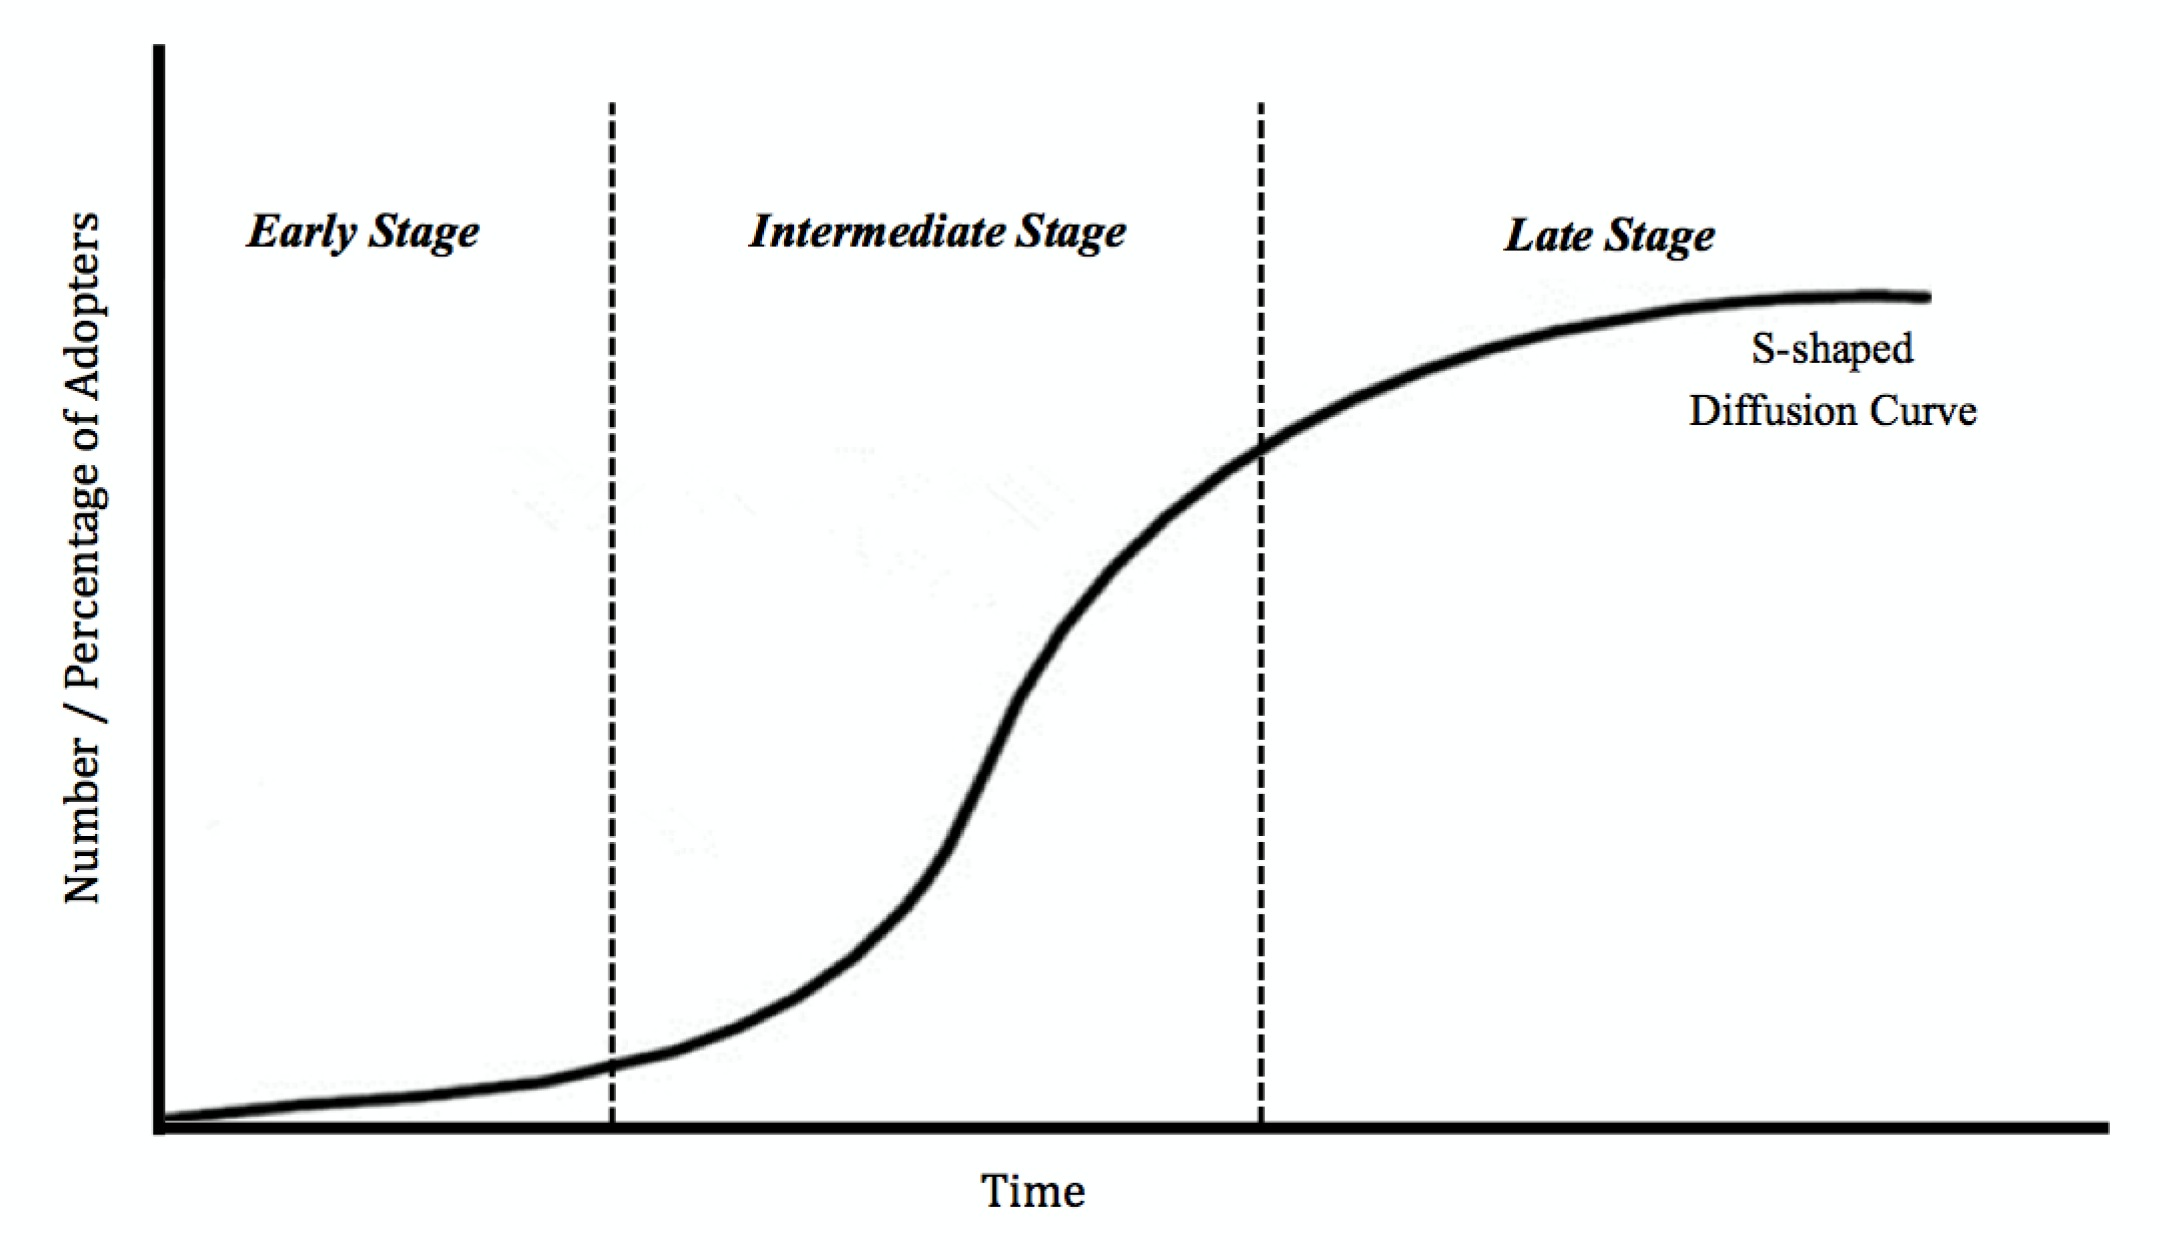
\includegraphics[scale=0.15]{peer_effects_and_diffusion_curve.jpg}
\caption{Peer Effects at Different Stages of the Diffusion Process}
\label{Fig: peer effects diffusion curve}
\end{figure}

\begin{figure}[h!]
\centering
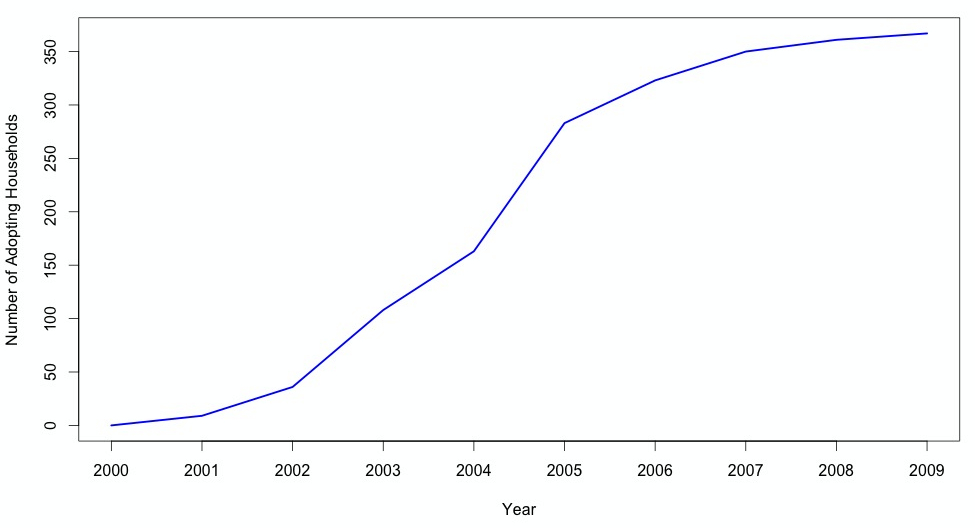
\includegraphics[scale=0.35]{Diffusion_curve_AS.jpg}
\caption{\textbf{Diffusion of the New Crop in the Chinese Villages}}
\label{Fig: diffusion curve AS}
\end{figure}

\begin{figure}[h!]
\centering
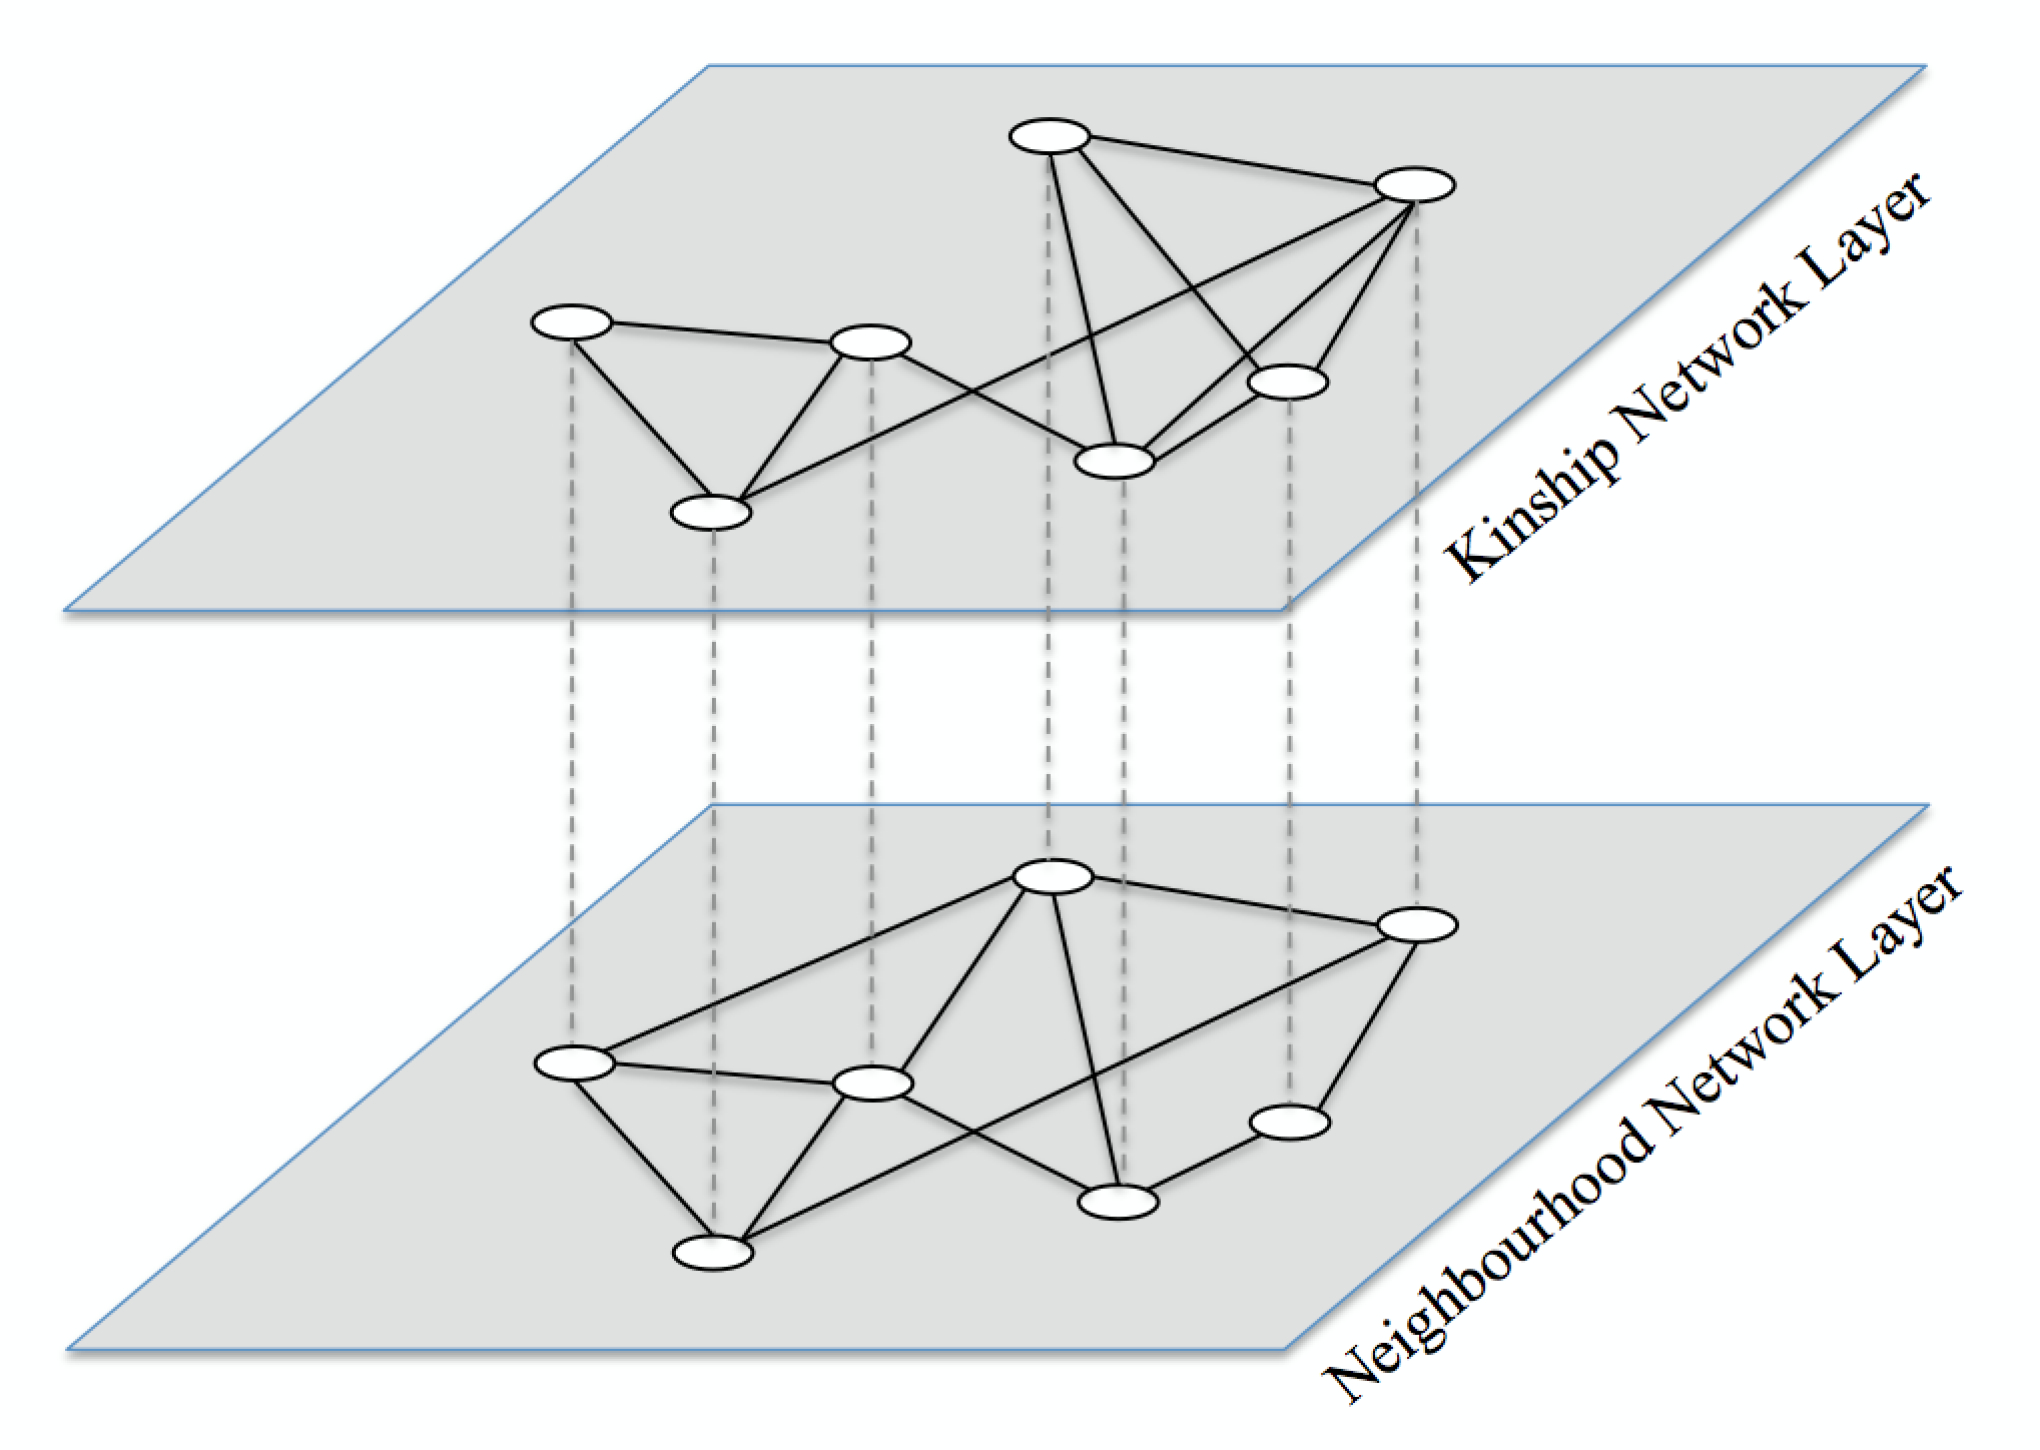
\includegraphics[scale=0.25]{two-layer_network.jpg}
\caption{Two-layer Multiplex Network}
\label{Fig: two-layer network}
\end{figure}

\begin{figure}[h!]
\centering
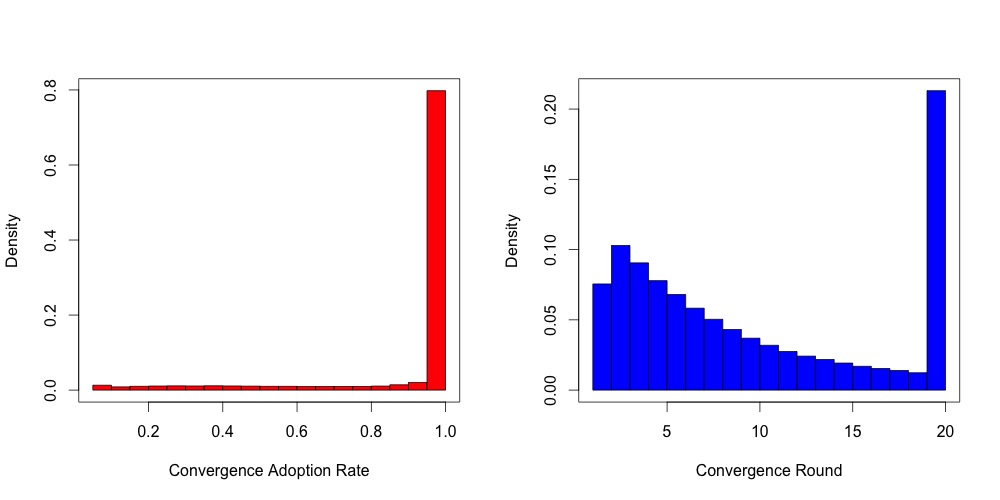
\includegraphics[scale=0.35]{Hist_conv_adp_and_round_pos.jpg}
\caption{\textbf{Histogram of Convergence Adoption Rates and Convergence Rounds (Positive Externality Effect)}}
\label{Fig: hist conv adp and round pos}
\end{figure}

\begin{figure}[h!]
\centering
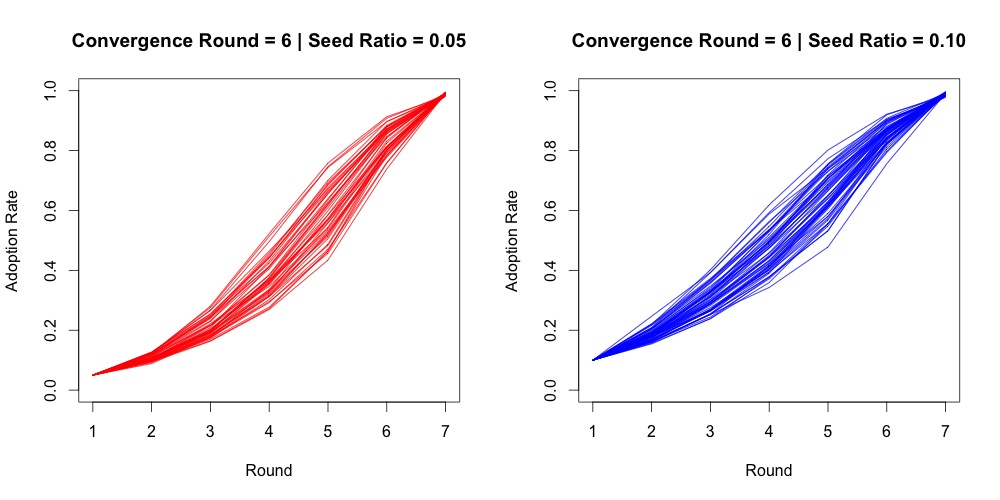
\includegraphics[scale=0.35]{S-shape_curves_round_6_pos.jpg}
\caption{S-shaped Diffusion Curves (Convergence Round = 6)}
\label{Fig: s-shaped curves round=6}
\end{figure}

\begin{figure}[h!]
\centering
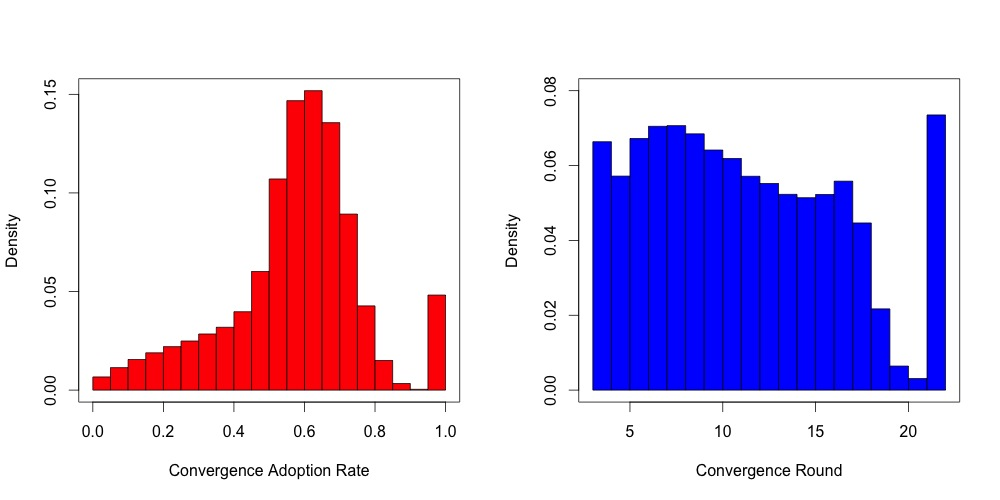
\includegraphics[scale=0.35]{Hist_conv_adp_and_round_neg.jpg}
\caption{Histogram of Convergence Adoption Rates and Convergence Rounds (Negative Externality Effect)}
\label{Fig: hist conv adp and round neg}
\end{figure}

\begin{figure}[h!]
\centering
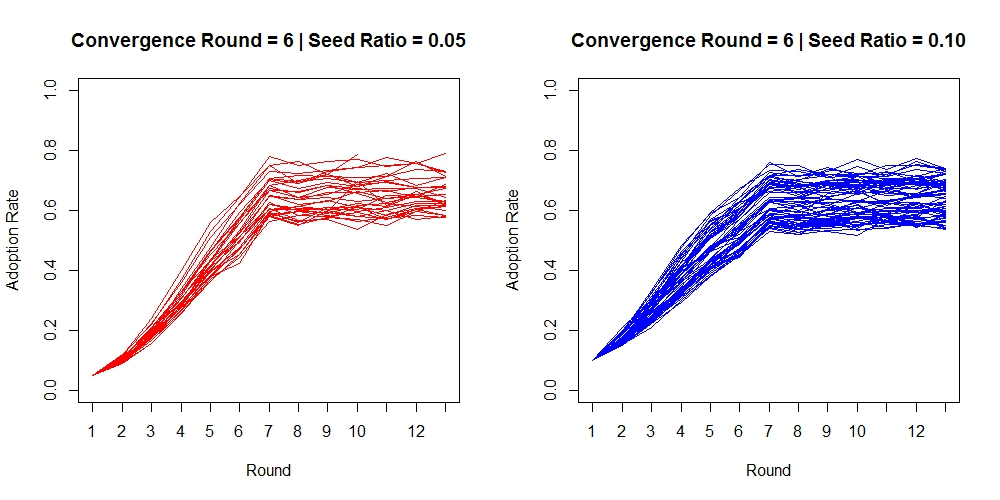
\includegraphics[scale=0.35]{Fluctuating_curves_round_6_neg.jpg}
\caption{Fluctuating Diffusion Curves (Convergence Round = 6)}
\label{Fig: fluctuating curves round=6}
\end{figure}


%%%%%%%%%%%%%%%%%%%%%%%%%%%%%%%%%%%
%%                               %%
%% Tables                        %%
%%                               %%
%%%%%%%%%%%%%%%%%%%%%%%%%%%%%%%%%%%

%% Use of \listoftables is discouraged.
%%
\section*{Tables}
\begin{table}[h!]
\caption{Regression for Adoption Speeds at Different Diffusion Levels (Positive Externality Effect)}
\label{Tab: reg adoption speed pos}
\resizebox{\linewidth}{!}{
\begin{tabular}{l D{.}{.}{5}@{} D{.}{.}{5}@{} D{.}{.}{5}@{} D{.}{.}{5}@{} D{.}{.}{5}@{} D{.}{.}{5}@{} D{.}{.}{5}@{} }
\toprule
& \multicolumn{1}{c}{Model 1} & \multicolumn{1}{c}{Model 2} & \multicolumn{1}{c}{Model 3} & \multicolumn{1}{c}{Model 4} & \multicolumn{1}{c}{Model 5} & \multicolumn{1}{c}{Model 6} & \multicolumn{1}{c}{Model 7} \\
& \multicolumn{1}{c}{(30\%)$^{*}$} & \multicolumn{1}{c}{(40\%)} & \multicolumn{1}{c}{(50\%)} & \multicolumn{1}{c}{(60\%)} & \multicolumn{1}{c}{(70\%)} & \multicolumn{1}{c}{(80\%)} & \multicolumn{1}{c}{(90\%)} \\
\midrule
(Intercept)                       & -0.53 & -0.50 & -0.47 & -0.45 & -0.43 & -0.32 & -0.32 \\
Number of Households                   & 0.01  & 0.01  & 0.01  & 0.01  & 0.01  & 0.01  & 0.01  \\
Ratio of Seed Adopters               & 0.90  & 0.84  & 0.81  & 0.80  & 0.78  & 0.57  & 0.57  \\
Experience Coefficient            & 2.04  & 2.02  & 2.01  & 1.99  & 1.94  & 1.54  & 1.54  \\
Externality Threshold             & -0.18 & -0.21 & -0.23 & -0.25 & -0.26 & -0.28 & -0.28 \\
\% of Neighbours to Connect in WS & 3.23  & 3.24  & 3.23  & 3.21  & 3.16  & 2.53  & 2.53  \\
Rewiring Probability in ER        & -0.15 & -0.14 & -0.12 & -0.10 & -0.08 & 0.09  & 0.09  \\
\midrule
R$^2$                             & 0.75      & 0.78        & 0.80        & 0.80        & 0.80        & 0.72        & 0.72        \\
\hline
\bottomrule
\multicolumn{8}{l}{\small{$^*$ The adoption rate level for diffusion speed in the present regression. This is the same for Table \ref{Tab: reg peer effects average degree pos}, \ref{Tab: reg peer effects clustering coefficient pos} and \ref{Tab: reg peer effects average path length pos}.}}
%\multicolumn{8}{l}{\small{\dag All effect sizes were significantly larger than the minimally meaningful effect of 0.1 standard deviations.}}
\end{tabular}
}
\end{table}

\begin{table}[h!]
\caption{Regression on Convergence Adoption Rate and Convergence Speed (Negative Externality Effect)}
\resizebox{0.8\linewidth}{!}{
\label{Tab: reg adoption rate neg}
\begin{tabular}{l D{.}{.}{15}@{} D{.}{.}{15}@{} }
\toprule
& \multicolumn{1}{c}{Model 1} & \multicolumn{1}{c}{Model 2} \\
& \multicolumn{1}{c}{(Conv. Adp. Rate)} & \multicolumn{1}{c}{(Conv. Speed)} \\
\midrule
(Intercept)                       & 0.90  & -0.31 \\
Number of Households                   & 0.00  & 0.01  \\
Ratio of Seed Adopters               & 0.17  & 0.57  \\
Experience Coefficient            & 0.19  & 1.53  \\
Externality Threshold             & -0.05 & -0.28 \\
\% of Neighbours to Connect in WS & 0.39  & 2.53  \\
Rewiring Probability in ER        & -0.02 & 0.06  \\
\midrule
R$^2$                             & 0.11        & 0.72        \\
\bottomrule
\end{tabular}
}
\end{table}

\begin{table}[h!]
\caption{Correlations between Network Characteristics (Positive Externality Effect)}
\label{Tab: correlation network characteristics pos}
\resizebox{0.9\linewidth}{!}{
\begin{tabular}{l D{.}{.}{5}@{} D{.}{.}{5}@{} D{.}{.}{5}@{} D{.}{.}{5}@{} D{.}{.}{5}@{} D{.}{.}{5}@{} D{.}{.}{5}@{} D{.}{.}{5}@{} }
\toprule
&(Var 1) & (Var 2) & (Var 3) &  (Var 4) & (Var 5) & (Var 6) & (Var 7) & (Var 8)\\ 
\midrule
$WS_f$ & 1 &  &  &  &  &  &  & \\ 
Avg. Dg. of Kin. & 0.65 & 1 &  &  &  &  &  &  \\ 
Clu. Coef. of Kin. & 0.83 & 0.69 & 1 &  &  &  &  &  \\ 
APL of Kin. & -0.73 & -0.64 & -0.86 & 1 &  &  &  & \\ 
$ER_{prob}$ &  &  &  &  & 1 &  &  &  \\ 
Avg. Dg. of Nei. &  &  &   &  & 0.49 & 1 &  &  \\ 
Clu. Coef. of Nei. &  &  &  &  & 0.71 & 0.43 & 1 &  \\
APL of Nei. &  &  &  & & -0.65 & -0.76 & -0.58 & 1 \\
\bottomrule
\end{tabular}
}
\end{table}

\begin{table}[h!]
\caption{Peer Effects and Average Degree (Positive Externality Effect)}
\label{Tab: reg peer effects average degree pos}
\resizebox{\linewidth}{!}{
\begin{tabular}{l D{.}{.}{5}@{} D{.}{.}{5}@{} D{.}{.}{5}@{} D{.}{.}{5}@{} D{.}{.}{5}@{} D{.}{.}{5}@{} D{.}{.}{5}@{} }
\toprule
& \multicolumn{1}{c}{Model 1} & \multicolumn{1}{c}{Model 2} & \multicolumn{1}{c}{Model 3} & \multicolumn{1}{c}{Model 4} & \multicolumn{1}{c}{Model 5} & \multicolumn{1}{c}{Model 6} & \multicolumn{1}{c}{Model 7} \\
& \multicolumn{1}{c}{(30\%)} & \multicolumn{1}{c}{(40\%)} & \multicolumn{1}{c}{(50\%)} & \multicolumn{1}{c}{(60\%)} & \multicolumn{1}{c}{(70\%)} & \multicolumn{1}{c}{(80\%)} & \multicolumn{1}{c}{(90\%)} \\
\midrule
(Intercept)                    & -0.07 & -0.05 & -0.04 & -0.03 & -0.01  & 0.02  & 0.02  \\
Number of Households           & -0.00 & 0.00        & 0.00  & 0.00  & 0.00  & 0.00  & 0.00  \\
Ratio of Seed Adopters                     & 0.90  & 0.84  & 0.81  & 0.80  & 0.78  & 0.57  & 0.57  \\
Experience Coefficient (Var 1)        & 0.87  & 0.99  & 1.07  & 1.08  & 1.02  & 0.74  & 0.74  \\
Externality Threshold (Var 2)         & -0.16 & -0.19 & -0.21 & -0.23 & -0.23 & -0.22 & -0.22 \\
Average Degree of Kin. (Var 3)      & 0.01  & 0.01  & 0.02  & 0.02  & 0.01  & 0.01  & 0.01  \\
Average Degree of Nei. (Var 4) & -0.00       & 0.00        & 0.00        & 0.00    & 0.00  & 0.01  & 0.01  \\
Var 1 $\times$ Var 3                  & 0.12  & 0.10  & 0.10  & 0.09  & 0.09  & 0.08  & 0.08  \\
Var 2 $\times$ Var 4             & -0.01 & -0.00 & -0.00 & -0.00 & -0.00 & -0.01 & -0.01 \\
\midrule
R$^2$                          & 0.80        & 0.81        & 0.82        & 0.82        & 0.82        & 0.75        & 0.75        \\
\bottomrule
\end{tabular}
}
\end{table}

\begin{table}[h!]
\caption{Peer Effects and Clustering Coefficient (Positive Externality Effect)}
\label{Tab: reg peer effects clustering coefficient pos}
\resizebox{\linewidth}{!}{
\begin{tabular}{l D{.}{.}{5}@{} D{.}{.}{5}@{} D{.}{.}{5}@{} D{.}{.}{5}@{} D{.}{.}{5}@{} D{.}{.}{5}@{} D{.}{.}{5}@{} }
\toprule
\hline
& \multicolumn{1}{c}{Model 1} & \multicolumn{1}{c}{Model 2} & \multicolumn{1}{c}{Model 3} & \multicolumn{1}{c}{Model 4} & \multicolumn{1}{c}{Model 5} & \multicolumn{1}{c}{Model 6} & \multicolumn{1}{c}{Model 7} \\
& \multicolumn{1}{c}{(30\%)} & \multicolumn{1}{c}{(40\%)} & \multicolumn{1}{c}{(50\%)} & \multicolumn{1}{c}{(60\%)} & \multicolumn{1}{c}{(70\%)} & \multicolumn{1}{c}{(80\%)} & \multicolumn{1}{c}{(90\%)} \\
\midrule
(Intercept)                    & -0.17 & -0.17 & -0.17 & -0.16 & -0.15 & -0.08 & -0.08 \\
Number of Households           & 0.00  & 0.00  & 0.00  & 0.00  & 0.00  & 0.00  & 0.00  \\
Ratio of Seed Adopters                     & 0.91  & 0.84  & 0.81  & 0.80  & 0.78  & 0.57  & 0.57  \\
Experience Coefficient (Var 1)        & 0.21  & 0.35  & 0.43  & 0.45  & 0.41  & 0.31  & 0.31  \\
Externality Threshold (Var 2)         & -0.18 & -0.20 & -0.21 & -0.22 & -0.23 & -0.25 & -0.25 \\
Clustering Coefficient of Kin. (Var 3)     & 0.12  & 0.22  & 0.29  & 0.31  & 0.30  & 0.24  & 0.24  \\
Clustering Coefficient of Nei. (Var 4) & -0.10   & -0.03      & 0.04        & 0.07    & 0.12   & 0.22  & 0.22  \\
Var 1 $\times$ Var 3                  & 7.06  & 6.47  & 6.10  & 5.9  & 5.80  & 4.77  & 4.77  \\
Var 2 $\times$ Var 4           & -0.00       & -0.08       & -0.16  & -0.20 & -0.24 & -0.25 & -0.25 \\
\midrule
R$^2$                          & 0.70        & 0.72        & 0.74        & 0.75        & 0.75        & 0.68        & 0.68        \\
\bottomrule
\end{tabular}
}
\end{table}

\begin{table}[h!]
\caption{Peer Effects and Average Path Length (Positive Externality Effect)}
\label{Tab: reg peer effects average path length pos}
\resizebox{\linewidth}{!}{
\begin{tabular}{l D{.}{.}{5}@{} D{.}{.}{5}@{} D{.}{.}{5}@{} D{.}{.}{5}@{} D{.}{.}{5}@{} D{.}{.}{5}@{} D{.}{.}{5}@{} }
\toprule
& \multicolumn{1}{c}{Model 1} & \multicolumn{1}{c}{Model 2} & \multicolumn{1}{c}{Model 3} & \multicolumn{1}{c}{Model 4} & \multicolumn{1}{c}{Model 5} & \multicolumn{1}{c}{Model 6} & \multicolumn{1}{c}{Model 7} \\
& \multicolumn{1}{c}{(30\%)} & \multicolumn{1}{c}{(40\%)} & \multicolumn{1}{c}{(50\%)} & \multicolumn{1}{c}{(60\%)} & \multicolumn{1}{c}{(70\%)} & \multicolumn{1}{c}{(80\%)} & \multicolumn{1}{c}{(90\%)} \\
\midrule
(Intercept)                    & -0.18 & -0.08 & -0.01       & 0.03    & 0.06  & 0.23  & 0.23  \\
Number of Households           & 0.00  & 0.00  & 0.00  & 0.00  & 0.00  & 0.00  & 0.00  \\
Ratio of Seed Adopters                     & 0.90  & 0.84  & 0.81  & 0.80  & 0.79  & 0.57  & 0.57  \\
Experience Coefficient (Var 1)        & 4.29  & 4.11  & 3.99  & 3.91  & 3.84  & 3.05  & 3.05  \\
Externality Threshold (Var 2)         & -0.25 & -0.30 & -0.34 & -0.36 & -0.39 & -0.50 & -0.50 \\
APL of Kin. (Var 3)     & 0.01  & -0.01 & -0.02 & -0.02 & -0.02 & -0.02 & -0.02 \\
APL of Nei. (Var 4) & 0.00        & -0.01       & -0.02  & -0.02 & -0.03 & -0.07 & -0.07 \\
Var 1 $\times$ Var 3                  & -1.01 & -0.94 & -0.89 & -0.87 & -0.85 & -0.68 & -0.68 \\
Var 2 $\times$ Var 4             & 0.03   & 0.04  & 0.05  & 0.05  & 0.06  & 0.09  & 0.09  \\
\midrule
R$^2$                          & 0.67       & 0.69        & 0.71        & 0.72        & 0.72        & 0.65        & 0.65        \\
\bottomrule
\end{tabular}
}
\end{table}

\begin{table}[h!]
\caption{Peer Effects and Average Degree (Negative Externality Effect)}
\label{Tab: reg peer effects average degree neg}
\resizebox{0.8\linewidth}{!}{
\begin{tabular}{l D{.}{.}{15}@{} D{.}{.}{15}@{}}
\toprule
& \multicolumn{1}{c}{Model 1} & \multicolumn{1}{c}{Model 2} \\
& \multicolumn{1}{c}{(Conv. Adp. Rate)} & \multicolumn{1}{c}{(Conv. Speed)} \\
\midrule
(Intercept)              & 0.85  & 0.08  \\
Number of Households     & 0.00  & 0.00  \\
Ratio of Seed Adopters   & 0.50  & 0.34  \\
Experience Coefficient (Var 1)  & 0.50  & 0.90  \\
Externality Threshold (Var 2)   & -0.05 & -0.28 \\
Average Degree of Kin. (Var 3)  & 0.01  & 0.02  \\
Average Degree of Nei. (Var 4)  & 0.01  & -0.01 \\
Var 1 $\times$ Var 3 & -0.03 & 0.02  \\
Var 2 $\times$ Var 4 & -0.04 & 0.09  \\
\midrule
R$^2$                    & 0.11       & 0.74        \\
\bottomrule
\end{tabular}
}
\end{table}
 
\begin{table}[h!]
\caption{Peer Effects and Clustering Coefficient (Negative Externality Effect)}
\label{Tab: reg peer effects clustering coefficient neg}
\resizebox{0.8\linewidth}{!}{
\begin{tabular}{l D{.}{.}{15}@{} D{.}{.}{15}@{} }
\toprule
& \multicolumn{1}{c}{Model 1} & \multicolumn{1}{c}{Model 2} \\
& \multicolumn{1}{c}{(Conv. Adp. Rate)} & \multicolumn{1}{c}{(Conv. Speed)} \\
\midrule
(Intercept)                    & 0.78  & -0.18 \\
Number of Households           & 0.00  & 0.00  \\
Ratio of Seed Adopters         & 1.02  & 0.24  \\
Experience Coefficient (Var 1)         & 0.20  & 1.43  \\
Externality Threshold (Var 2)        & -0.05 & -0.28 \\
Clustering Coefficient of Kin. (Var 3) & 0.66  & 0.79  \\
Clustering Coefficient of Nei. (Var 4) & 0.00       & -0.08 \\
Var 1 $\times$ Var 3      & -3.29 & 1.29  \\
Var 2 $\times$ Var 4       & -0.10  & 0.72  \\
\midrule
R$^2$                          & 0.18       & 0.66        \\
\bottomrule
\end{tabular}
}
\end{table}

\begin{table}[h!]
\caption{Peer Effects and Average Path Length (Negative Externality Effect)}
\label{Tab: reg peer effects average path length neg}
\resizebox{0.8\linewidth}{!}{
\begin{tabular}{l D{.}{.}{15}@{} D{.}{.}{15}@{} }
\toprule
& \multicolumn{1}{c}{Model 1} & \multicolumn{1}{c}{Model 2} \\
& \multicolumn{1}{c}{(Conv. Adp. Rate)} & \multicolumn{1}{c}{(Conv. Speed)} \\
\midrule
(Intercept)                    & 1.28  & 0.04  \\
Number of Households           & 0.00  & 0.00  \\
Ratio of Seed Adopters         & -0.98 & 0.97  \\
Experience Coefficient (Var 1)        & -0.44 & 2.87  \\
Externality Threshold (Var 2)         & -0.05 & -0.28 \\
APL. of Kin. (Var 3) & -0.10 & -0.10 \\
APL. of Nei. (Var 4) & -0.04 & 0.08 \\
Var 1 $\times$ Var 3       & 0.52  & -0.18 \\
Var 2 $\times$ Var 4      & 0.28  & -0.59 \\
\midrule
R$^2$                          & 0.22       & 0.63        \\
\bottomrule
\end{tabular}
}
\end{table}
\fi
%%%%%%%%%%%%%%%%%%%%%%%%%%%%%%%%%%%
%%                               %%
%% Additional Files              %%
%%                               %%
%%%%%%%%%%%%%%%%%%%%%%%%%%%%%%%%%%%

\end{backmatter}
\end{document}
